\documentclass[10pt]{article}
\usepackage[a4paper,margin=25mm]{geometry}
\usepackage{amsmath,booktabs,graphicx}
\usepackage{tikz}
\usetikzlibrary{arrows.meta,positioning}
\usepackage[hidelinks]{hyperref}
% Generated by tools/export_research_draft_evidence.py; do not edit.
\newcommand{\CrossExpanded}{229746}
\newcommand{\CrossObservations}{862428}
\newcommand{\CrossCost}{42}
\newcommand{\JointCalls}{16}
\newcommand{\SmokeExpanded}{2}
\newcommand{\SmokeUpload}{3746844664}
\newcommand{\DelayConnections}{5980}
\newcommand{\EntryWL}{10749}
\newcommand{\EntryCPD}{9.67608}
\newcommand{\EntryExpanded}{96811142}
\newcommand{\StopExpanded}{36318898}
\newcommand{\StopUpstreamReduction}{95.21}
\newcommand{\StopTotalReduction}{62.48}
\newcommand{\FineFlatWL}{10771}
\newcommand{\FineFlatCPD}{9.69287}
\newcommand{\FineFlatIterations}{9}
\newcommand{\FineDownWL}{10722}
\newcommand{\FineDownCPD}{9.91429}
\newcommand{\FineDownIterations}{15}
\newcommand{\LocalOrderWL}{10954}
\newcommand{\LocalOrderCPD}{9.65946}
\newcommand{\LocalOrderIterations}{9}
\newcommand{\CleanupWL}{10684}
\newcommand{\CleanupBeforeWL}{10749}
\newcommand{\CleanupCPD}{9.67608}
\newcommand{\CleanupAccepted}{9}
\newcommand{\CleanupWireReduction}{65}
\newcommand{\CleanupExpandedIncrease}{60.77}
\newcommand{\CleanupWLDelta}{10.55}
\newcommand{\ZeroSeedWL}{9521}
\newcommand{\ZeroSeedCPD}{10.2293}
\newcommand{\ZeroSeedWLDelta}{-1.48}
\newcommand{\ZeroSeedCPDDelta}{6.55}
\newcommand{\MidSeedWL}{9929}
\newcommand{\MidSeedCPD}{9.63263}
\newcommand{\MidSeedWLDelta}{2.74}
\newcommand{\MidSeedCPDDelta}{0.34}
\newcommand{\SpanWL}{10529}
\newcommand{\SpanCPD}{9.81527}
\newcommand{\SpanWLReduction}{220}
\newcommand{\SpanCompatibleArtifacts}{50}
\newcommand{\TraceAccepted}{11122}
\newcommand{\TraceCompatibleArtifacts}{50}
\newcommand{\TraceFinalCapped}{15}
\newcommand{\TraceBelowFinalCap}{9}
\newcommand{\TraceCorruptions}{6}
\newcommand{\TraceMidAccepted}{11264}
\newcommand{\TraceMidCapped}{48}
\newcommand{\TraceMidBelowCap}{27}
\newcommand{\TraceMidExampleBranch}{786}
\newcommand{\FeedbackWL}{9809}
\newcommand{\FeedbackCPD}{9.78317}
\newcommand{\FeedbackSupplemental}{52}
\newcommand{\FeedbackUnchanged}{46}
\newcommand{\HardwareNoInputDelay}{7}
\newcommand{\HardwareNoOutputDelay}{3}
\newcommand{\HardwareRequestedMHz}{300.0}
\newcommand{\HardwareReportedMHz}{205.7}
\newcommand{\HardwareDataMHz}{205}
\newcommand{\HardwareWNS}{-1.528}
\newcommand{\HardwareFailingEndpoints}{42516}
\newcommand{\HardwarePointers}{35}
\newcommand{\CommitUnbankedLUT}{108996}
\newcommand{\CommitBankedLUT}{144002}
\newcommand{\CommitLUTIncrease}{32.1}
\newcommand{\CommitFFIncrease}{27.0}
\newcommand{\LocalGuardWL}{9762}
\newcommand{\LocalGuardCPD}{10.06}
\newcommand{\LocalGuardWLDelta}{1.01}
\newcommand{\LocalGuardCPDDelta}{4.79}
\newcommand{\LocalGuardSupplemental}{4}
\newcommand{\LocalGuardCompatibleArtifacts}{70}
\newcommand{\LocalGuardSlowerEvents}{4}
\newcommand{\LocalGuardSlowerConnections}{37}
\newcommand{\LocalGuardMaxIncrease}{475}
\newcommand{\NetTrialParentWL}{9762}
\newcommand{\NetTrialParentCPD}{10.06}
\newcommand{\NetTrialStagedWL}{9902}
\newcommand{\NetTrialStagedCPD}{9.6313}
\newcommand{\NetTrialGuardedWL}{9919}
\newcommand{\NetTrialGuardedCPD}{9.63263}
\newcommand{\NetTrialQueries}{91}
\newcommand{\NetTrialHashFields}{202}
\newcommand{\NetTrialPublished}{1}
\newcommand{\NetTrialRejected}{4}
\newcommand{\NetTrialDiscardedVersions}{445}
\newcommand{\NetTrialMutations}{10}
\newcommand{\NetTrialCompatible}{70}
\newcommand{\OrdinaryBulkWL}{9929}
\newcommand{\OrdinaryBulkCPD}{9.63263}
\newcommand{\OrdinaryDispatchWL}{10026}
\newcommand{\OrdinaryDispatchCPD}{10.0142}
\newcommand{\OrdinarySerialWL}{9443}
\newcommand{\OrdinarySerialCPD}{10.2508}
\newcommand{\OrdinaryCorruptions}{27}
\newcommand{\OrdinaryCompatible}{70}
\newcommand{\QualityFrontierEntries}{39}
\newcommand{\QualityFrontierPoints}{25}
\newcommand{\VPRFrozenFiles}{17526}
\newcommand{\VPRCompiledUnits}{304}
\newcommand{\VPRDependencyInputs}{1701}
\newcommand{\VPRNativeRepeats}{5}
\newcommand{\VPRBaselineWL}{9664}
\newcommand{\VPRBaselineCPD}{9.60037}
\newcommand{\VPRHookNativeRepeats}{5}
\newcommand{\VPRHookEpochs}{10}
\newcommand{\VPRHookRows}{19200}
\newcommand{\VPRSetupCalls}{4743}
\newcommand{\VPRSetupEpochs}{21}
\newcommand{\VPRWholeReset}{4383}
\newcommand{\VPRPartialPrune}{330}
\newcommand{\VPRFullPrune}{30}
\newcommand{\VPRRetainedFlags}{5383}
\newcommand{\PresentLegacyWL}{9929}
\newcommand{\PresentLegacyCPD}{9.63263}
\newcommand{\PresentLegacyCrossings}{450}
\newcommand{\PresentLegacyEpochs}{10}
\newcommand{\PresentSlowWL}{9736}
\newcommand{\PresentSlowCPD}{9.6716}
\newcommand{\PresentSlowCrossings}{448}
\newcommand{\PresentSlowEpochs}{23}
\newcommand{\PresentWarmWL}{9512}
\newcommand{\PresentWarmCPD}{9.54931}
\newcommand{\PresentWarmCrossings}{454}
\newcommand{\PresentWarmEpochs}{22}
\newcommand{\PresentBaselineCrossings}{484}
\newcommand{\PresentWarmExpanded}{69388394}
\newcommand{\PresentWarmExpansionRatio}{2.08}
\newcommand{\LegalRetainedOccurrences}{1788}
\newcommand{\LegalRetentionWL}{9973}
\newcommand{\LegalRetentionCPD}{9.91446}
\newcommand{\LegalRetentionExpanded}{28394845}
\newcommand{\LegalRetentionEpochs}{21}
\newcommand{\FixedDiffeqWL}{8740}
\newcommand{\FixedDiffeqBaselineWL}{8639}
\newcommand{\FixedDiffeqCPD}{7.59047}
\newcommand{\FixedDiffeqBaselineCPD}{7.61372}
\newcommand{\FixedAluWL}{7376}
\newcommand{\FixedAluCPD}{9.49596}
\newcommand{\FixedAluBaselineCPD}{9.49369}
\newcommand{\PersistentFreshMedian}{232.42}
\newcommand{\PersistentMedian}{63.18}
\newcommand{\PersistentPairedRatio}{3.73}
\newcommand{\PersistentRatioMin}{3.59}
\newcommand{\PersistentRatioMax}{3.81}
\newcommand{\CriticalityShiftWL}{9749}
\newcommand{\CriticalityShiftCPD}{9.68003}
\newcommand{\CriticalityShiftCrossings}{448}
\newcommand{\CriticalityShiftEpochs}{23}
\newcommand{\CriticalityShiftExpanded}{70410074}
\newcommand{\BankedSnapshotWNS}{-2.014}
\newcommand{\BankedSnapshotTNS}{-22733.928}
\newcommand{\BankedSnapshotFailingEndpoints}{46868}
\newcommand{\BankedSnapshotWorstData}{4.831}
\newcommand{\BankedSnapshotWorstRoute}{3.356}
\newcommand{\BankedReportedMHz}{187.0}
\newcommand{\BankedDataMHz}{187}
\newcommand{\BankedPointers}{39}
\newcommand{\BankedLUT}{249641}
\newcommand{\BankedFF}{376476}
\newcommand{\BankedBRAM}{422}
\newcommand{\BankedURAM}{0}
\newcommand{\BankedDSP}{63}
\newcommand{\BankedDRCWarnings}{314}
\newcommand{\BankedDRCAdvisories}{5}
\newcommand{\BankedNoInputDelay}{7}
\newcommand{\BankedNoOutputDelay}{3}
\newcommand{\StaticSourceRemoteReads}{16909117}
\newcommand{\StaticDestinationRemoteReads}{1317058}
\newcommand{\StaticRemoteReduction}{92.21}
\newcommand{\StaticMovedOccurrences}{4444}
\newcommand{\StaticLogicalMovedBytes}{1476644}
\newcommand{\StaticPlacementWL}{9929}
\newcommand{\StaticPlacementCPD}{9.63263}
\newcommand{\InitialNativeWL}{9665}
\newcommand{\InitialNativeCPD}{9.69023}
\newcommand{\InitialNativeCrossings}{448}
\newcommand{\InitialObservedTasks}{1920}
\newcommand{\InitialQMin}{42123}
\newcommand{\InitialQMax}{64880}
\newcommand{\InitialQDistinct}{22}
\newcommand{\ReceivedNativeSeeds}{1516375}
\newcommand{\ReceivedNativeRequests}{56320}
\newcommand{\CreditNativeTasks}{11264}
\newcommand{\CreditEntryStalls}{3093}
\newcommand{\CreditByteStalls}{265}
\newcommand{\CreditByteLimit}{2076}
\newcommand{\AdaptiveNativeBackpressure}{2025}
\newcommand{\AdaptiveNativeRemote}{5124816}
\newcommand{\AdaptiveNativeWindows}{5707}
\newcommand{\HBMFailingSetup}{365}
\newcommand{\HBMWorstSlack}{-0.216}
\newcommand{\KernelFailingSetup}{46503}
\newcommand{\FanoutBulkWL}{9996}
\newcommand{\FanoutBulkCPD}{9.75744}
\newcommand{\FanoutSerialWL}{9420}
\newcommand{\FanoutSerialCPD}{9.74681}
\newcommand{\FullSeedFanoutWL}{10064}
\newcommand{\FullSeedFanoutCPD}{9.78266}
\newcommand{\APIJournalEntries}{49069223}
\newcommand{\APIProposalPhases}{13950}
\newcommand{\APIResourceCalls}{269360030}
\newcommand{\APICostCalls}{248635515}
\newcommand{\BusSkewNumericConstraints}{229}
\newcommand{\BusSkewMinimumSlack}{1.49}
\newcommand{\WarmFanoutWL}{9622}
\newcommand{\WarmFanoutCPD}{9.65646}
\newcommand{\WarmFanoutCrossings}{446}
\newcommand{\APICoveredTotalEntries}{245346115}
\newcommand{\APICoveredTotalPhases}{69750}
\newcommand{\APICoveredTotalStale}{13430}
\newcommand{\APICoverageMatchedArtifacts}{235}
\newcommand{\FourLayerSourceFiles}{17526}
\newcommand{\FourLayerTranslationUnits}{304}
\newcommand{\STARepairBestWL}{12017}
\newcommand{\STARepairBestCPD}{10.4694}
\newcommand{\SlackCheckpointWL}{11606}
\newcommand{\SlackCheckpointCPD}{10.5304}
\newcommand{\SlackCheckpointCrossings}{998}
\newcommand{\SlackExFinalWL}{11496}
\newcommand{\SlackExFinalCPD}{10.5304}
\newcommand{\SlackExFinalCrossings}{999}
\newcommand{\SlackExFinalAccepted}{56}
\newcommand{\SlackExNativeCalls}{174}
\newcommand{\SlackDiffeqWL}{11336}
\newcommand{\SlackDiffeqCPD}{7.74031}
\newcommand{\SlackDiffeqCrossings}{727}
\newcommand{\SlackDiffeqAccepted}{60}
\newcommand{\SlackAluWL}{9422}
\newcommand{\SlackAluCPD}{10.3951}
\newcommand{\SlackAluCrossings}{886}
\newcommand{\SlackAluAccepted}{112}
\newcommand{\RefreshedExWL}{11397}
\newcommand{\RefreshedExCPD}{10.4526}
\newcommand{\RefreshedExCrossings}{991}
\newcommand{\RefreshedExAccepted}{3}
\newcommand{\RefreshedDiffWL}{11206}
\newcommand{\RefreshedDiffCPD}{7.74031}
\newcommand{\RefreshedDiffCrossings}{727}
\newcommand{\RefreshedDiffAccepted}{0}
\newcommand{\RefreshedAluWL}{9424}
\newcommand{\RefreshedAluCPD}{10.3951}
\newcommand{\RefreshedAluCrossings}{886}
\newcommand{\RefreshedAluAccepted}{0}
\newcommand{\CompoundExSeconds}{4216.6}
\newcommand{\CompoundDiffSeconds}{5495.2}
\newcommand{\CompoundAluSeconds}{4527.1}
\newcommand{\TailStaticSeconds}{1259.4}
\newcommand{\TailStaticBackpressure}{2233}
\newcommand{\TailStaticRemoteReads}{407075499}
\newcommand{\TailAdaptiveSeconds}{1501.3}
\newcommand{\TailAdaptiveBackpressure}{804}
\newcommand{\TailAdaptiveRemoteReads}{431550917}
\newcommand{\LeanStartLUTDelta}{34215}
\newcommand{\LeanStartFFDelta}{29515}
\newcommand{\LeanStartDSPDelta}{12}
\newcommand{\AdaptiveRefinementSeconds}{3609.4}
\newcommand{\HashMedianTimeReduction}{8.05}
\newcommand{\HashMinimumTimeReduction}{7.92}
\newcommand{\HashMaximumTimeReduction}{10.53}
\newcommand{\DiffeqHashMedianReduction}{7.49}
\newcommand{\DiffeqHashMinimumReduction}{4.79}
\newcommand{\DiffeqHashMaximumReduction}{8.27}
\newcommand{\AluHashMedianReduction}{7.44}
\newcommand{\AluHashMinimumReduction}{6.65}
\newcommand{\AluHashMaximumReduction}{10.52}
\newcommand{\PersistentPairRows}{%
1 & F/P & 225.54 & 60.53 & 3.73 \\
2 & P/F & 231.20 & 61.29 & 3.77 \\
3 & F/P & 240.60 & 63.18 & 3.81 \\
4 & P/F & 238.10 & 64.14 & 3.71 \\
5 & F/P & 232.42 & 64.71 & 3.59 \\
}
\newcommand{\SBScalingRows}{%
2 & 80 & 133800 & 0 & 11939 & 10.2564 \\
2 & 96 & 159132 & 0 & 11111 & 10.2836 \\
3 & 80 & 336312 & 90408 & 11615 & 10.4531 \\
3 & 96 & 409326 & 113752 & 10870 & 10.2814 \\
4 & 80 & 629232 & 271224 & 13735 & 11.2695 \\
4 & 96 & 773272 & 341256 & 12148 & 10.8438 \\
}
\newcommand{\SBPathRows}{%
2 & 80 & 994 & 926 & 0 & 0 & 598\\
2 & 96 & 1038 & 882 & 0 & 0 & 575\\
3 & 80 & 653 & 834 & 433 & 0 & 999\\
3 & 96 & 750 & 967 & 203 & 0 & 901\\
4 & 80 & 571 & 703 & 495 & 151 & 1266\\
4 & 96 & 708 & 930 & 244 & 38 & 1023\\
}
\newcommand{\DevelopmentQoRRows}{%
diffeq & 8639 & 8996 & 4.13\% & -0.03\% \\
alu4 & 7733 & 8353 & 8.02\% & -0.67\% \\
ex5p & 9664 & 10762 & 11.36\% & 2.28\% \\
}
\newcommand{\OwnerExchangeRows}{%
off/130 & 12215 & 10.5522 & 843 \\
off/318 & 12238 & 10.5522 & 842 \\
on/318 & 12028 & 10.4694 & 828 \\
}
\newcommand{\GateRows}{%
G1 & in\_progress & Not complete \\
G2 & in\_progress & Not complete \\
G3 & in\_progress & Not complete \\
G4 & in\_progress & Not complete \\
G5 & in\_progress & Not complete \\
G6 & in\_progress & Not complete \\
G7 & pending\_external\_hardware & Not complete \\
G8 & in\_progress & Not complete \\
}

\title{DieRoute: Multi-Die Routing with Partitioned Authority\\\large Evidence and Research Draft}
\author{Research draft; authorship and venue pending}
\date{15 October 2026}
\begin{document}
\maketitle
\begin{abstract}
DieRoute studies cross-die routing using SLL reservation, die-local resource
authority, versioned boundary summaries, and HBM placement. The prototype
reuses PersistRoute search and transactional commit infrastructure. We report
verified component behavior, native-graph snapshot searches, and actual compute
unit execution in hardware emulation. Separate resource buffers map three
owner shards to HBM groups 13, 14, and 15. These results establish bounded
functional properties of a serialized prototype. They do not establish an
asynchronous multi-owner architecture or board performance. On ex5p,
congestion-schedule calibration improves wirelength, timing and model crossing
counts, but fixed-setting diffeq validation fails wirelength and alu4 fails CPD. Full-cohort and
physical-acceleration requirements remain open.
This draft records the verified scope and remaining research gates.
\end{abstract}

\section{Problem and scope}
Cross-die connections couple local resource occupancy to scarce boundary
resources. The research objective is to route complete designs while preserving
native legality, timing and wirelength, and to obtain an independently measured
end-to-end accelerator benefit. PersistRoute provides the reused search,
versioned validation and commit substrate; reuse is not claimed as DieRoute
novelty. The proposed research contributions are SLL reservation and corridor
repair, single-owner resource state with boundary summaries, HBM/die mapping,
and criticality/congestion-aware migration. The latter contributions require
additional integration and ablation evidence.

\section{Preliminary related-work positioning}
Poolad et al. extend VTR for multi-die architecture modeling and optimization,
including inter-die connectivity and circuit-model exploration~\cite{multidie}.
Consequently, multi-die graph representation and architecture exploration alone
are insufficient as a proposed DieRoute contribution.
Their lookahead separates intra-die estimates from minimum crossing penalties;
die-aware heuristics and boundary-congestion awareness are also prior work.
The published lookahead uses static minimum-delay cut penalties; our current
source additionally evaluates a snapshot-specific node/stage suffix using
resource costs and feasibility. This observed mechanism difference is not a
novelty proof or matched performance comparison.
RWRoute provides commercial UltraScale+ timing-driven and partial routing with
a lightweight timing model~\cite{rwroute}. Native legality and comparison to a
strong commercial baseline remain necessary for this research.
Current official documentation also describes criticality-aware resource
sharing and configurable timing/length tradeoffs, while listing no hold-time
estimation in its described timing model~\cite{rwdocs}. These capabilities
and validation limits are comparison axes; documentation silence does not
prove protocol novelty. This documentation review is separate from the
2022 paper, whose body remains unreviewed here.
Official RapidWright release notes also list SLL tile support and SLR-crossing
optimizations in 2025.1.1, followed by initial Versal SLR-crossing support in
2025.2.0~\cite{rwrelease}. Cross-SLR awareness alone is therefore not a
distinguishing claim; these release entries do not establish implementation
equivalence or comparative performance.
Farkish and Jahanian study multithreaded PathFinder global routing~\cite{parallel}.
Parallel routing itself is therefore also prior work.
Selected pinned Potter source also separates routing, deferred net-usage
updates and congestion refresh with thread joins, and uses atomic node
occupancy~\cite{potterrepo}. Overlap tolerance and deferred synchronization
are therefore comparison axes. This bounded source inspection establishes
neither protocol equivalence nor DieRoute novelty or comparative speed.
Their method uses per-net mesh copies, global congestion updates, iteration
barriers and workload distribution by terminal count.

Huang et al. map routing search and network state spatially into hardware
and examine stochastic congestion management~\cite{spatial}.
Shen et al. use dynamically expanding subgraphs and GPU-friendly shortest
paths~\cite{gpu}. Their multi-net method groups independent subgraph boxes
while preserving the original serial net order, and combines them through
a virtual-source pseudo-net. Deterministic ordering and accelerator work
assignment are therefore also prior comparison axes. Zang et al. combine recursive ternary partitioning with
hybrid congestion updates for commercial-device parallel routing~\cite{commercialparallel}.
Hardware search, graph restriction, scheduling and cost updates therefore
form required comparison axes for DieRoute.

These preliminary references motivate focusing the research question on the
proposed state ownership and publication protocol, boundary reservation and mapped
hardware execution. This is an inference about useful comparison axes, not a
verified novelty claim. Review covers selected mechanism sections and author
introductions, with scope recorded separately for each source. RWRoute remains
reviewed at the metadata/abstract level. Comprehensive primary-source and
accelerator comparison are still required.

\section{Authority and search protocol}
For an electrical routing resource $r$, exactly one logical owner stores its
authoritative occupancy, history, version and membership. A boundary summary
is read-only information derived from that authority; it must not become a
second independent writer. Physical die membership and authority ownership
are separate concepts, particularly for resources spanning multiple dies.
The prototype uses a canonical owner within the membership set.

A proposal records each consumed resource observation and its version.
Publication requires compatible session/epoch identity, valid graph edges and
immutable admission policy, and current consumed versions. A failed proposal
must preserve all authority bytes. Multi-sink branches attach to the existing
net tree, and shared resources count once per net. These requirements apply
also to rejected search, malformed paths and late commit overflow.

The present banked implementation has three separate resource AXI interfaces
and shared tree, net and control state. Searches consume immutable authority
snapshots; commit follows under exclusive serialized handoff. The search and
commit compute units share the same device buffers. This implementation is a
functional step toward the architecture: independent buffers do not prove
concurrent writers, distributed ordering or asynchronous shadow coherence.

A separate CPU control varies the observer die used by speculative search:
legacy worker assignment, a source-die queue, or a destination-die queue.
All three use two workers, shadow synchronization every window and the
legacy congestion preset. Five repetitions per arm preserve all 41 core
route artifacts across modes; controller resource/version replay and task
receipt checks pass. Destination placement changes
\StaticMovedOccurrences{} task occurrences per run and records
\StaticLogicalMovedBytes{} logical envelope bytes. Remote-labelled shadow
read entries fall from \StaticSourceRemoteReads{} to
\StaticDestinationRemoteReads{} (\StaticRemoteReduction{}\%). This counts
observer-classified journal entries, not network bytes or physical PE
migration. All three native routes have wirelength \StaticPlacementWL{}
and CPD \StaticPlacementCPD{} ns, failing the strong baseline joint gate.
An encoded-transfer successor holds per-die byte and entry credits through
actual search completion, drains completed work on backpressure and
retains the original authority commit order. Three configurations complete
five ex5p runs each: no credit constraint, one in-flight entry per die, and
a \CreditByteLimit{}-byte limit. Each constrained run handles
\CreditNativeTasks{} transfers; the entry and byte limits respectively
cause \CreditEntryStalls{} and \CreditByteStalls{} backpressure events.
All credits return at completion and independent state/version, queue and
native-route checks pass, with the same failed baseline quality gate.
These limits cover encoded queued/in-flight payload, not total process memory.

A separate receiver observation completes five native runs, independently
reconstructing \ReceivedNativeSeeds{} decoded seed records across
\ReceivedNativeRequests{} task requests from the original CSR, controller
trees and STA outputs. Every node, hop count, seed cost and order is
checked, including seeds unused by the final branch. Routing artifacts
and quality remain unchanged.

A frozen CPU adaptive policy chooses source or sink execution using
criticality-weighted locality, authoritative boundary occupancy/history
and live byte/entry credits. Five native runs per arm compare it with
static destination placement at one credit per die and synchronization
every window. Independent replay verifies each decision's inputs, scores
and admission loads across \AdaptiveNativeWindows{} windows per run.
Backpressure events fall from \CreditEntryStalls{} to
\AdaptiveNativeBackpressure{}, while remote-labelled read entries rise
from \StaticDestinationRemoteReads{} to \AdaptiveNativeRemote{}.
Native WL and CPD are identical and still fail the strong baseline gate.
These count tradeoffs establish no network traffic or latency benefit;
independent full search-access enumeration and hardware queue transport
remain open.

A subsequent explicit view-API census completes five covered and five
control native runs. Each covered run checks \APIProposalPhases{} proposal
phases and \APIJournalEntries{} unique node occurrences against the
validation journal, with \APIResourceCalls{} resource calls and
\APICostCalls{} cost calls including diagnostic snapshot queries.
The five covered runs total \APICoveredTotalEntries{} unique occurrences,
\APICoveredTotalPhases{} phases and \APICoveredTotalStale{} stale/fresh
replays. Independent authority-value, coverage, tree and session checks
pass; \APICoverageMatchedArtifacts{} control artifacts match. A terminal
review stream-hashes the current referenced files, including large binary
logs, once. Both arms retain WL/CPD 9929/9.63263 ns and fail the quality
gate. This evidence covers explicit APIs, not arbitrary C++ pointer
accesses, a separate search rerun or physical traffic.

\begin{figure}[ht]
\centering
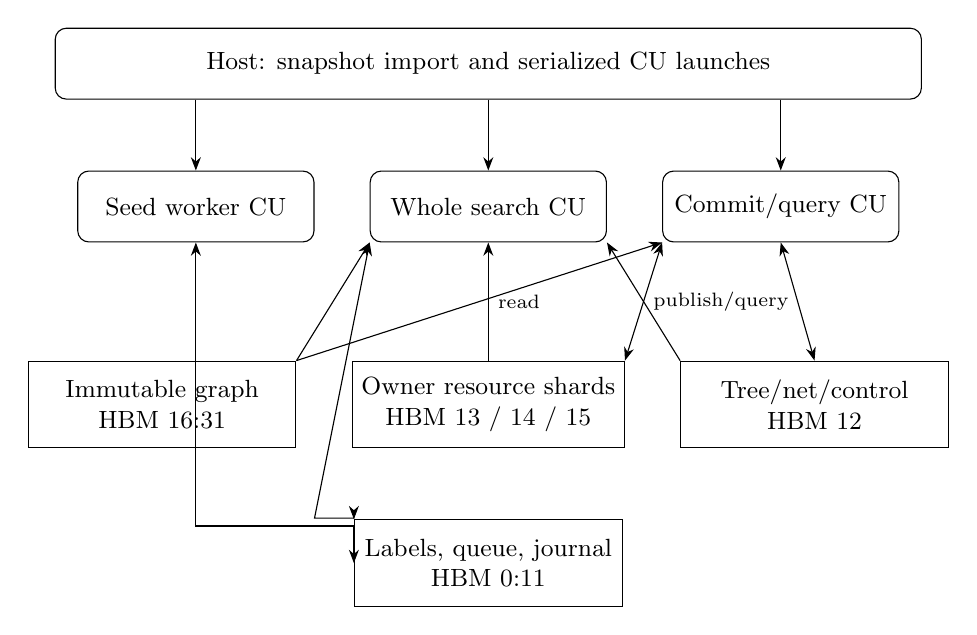
\begin{tikzpicture}[>=Stealth,font=\small,
cu/.style={draw,rounded corners,align=center,minimum width=30mm,minimum height=9mm},
mem/.style={draw,align=center,minimum width=34mm,minimum height=11mm}]
\node[cu,minimum width=110mm] (host) {Host: snapshot import and serialized CU launches};
\node[cu,below=9mm of host] (search) {Whole search CU};
\node[cu,left=7mm of search] (worker) {Seed worker CU};
\node[cu,right=7mm of search] (commit) {Commit/query CU};
\node[mem,below=15mm of search] (owners) {Owner resource shards\\HBM 13 / 14 / 15};
\node[mem,left=7mm of owners] (graph) {Immutable graph\\HBM 16:31};
\node[mem,right=7mm of owners] (authority) {Tree/net/control\\HBM 12};
\node[mem,below=9mm of owners] (scratch) {Labels, queue, journal\\HBM 0:11};
\draw[->] (host.south) -- (search.north);
\draw[->] (host.south -| worker.north) -- (worker.north);
\draw[->] (host.south -| commit.north) -- (commit.north);
\draw[->] (owners.north) -- node[right,font=\scriptsize]{read} (search.south);
\draw[<->] (commit.south west) -- node[right,font=\scriptsize]{publish/query} (owners.north east);
\draw[->] (graph.north east) -- (search.south west);
\draw[->] (graph.north east) -- (commit.south west);
\draw[->] (authority.north west) -- (search.south east);
\draw[<->] (authority.north) -- (commit.south);
\draw[<->] (worker.south) -- ++(0,-36mm) -| (scratch.west);
\draw[<->] (search.south west) -- ++(-7mm,-35mm) -| (scratch.north west);
\end{tikzpicture}
\caption{Verified buffer roles of the three-CU banked prototype. Lines show
logical accesses, not simultaneous traffic or independent authority writers.
Host launch ordering provides exclusive search/commit handoff.}
\label{fig:prototype}
\end{figure}

\section{Corridor selection and development variants}
The routing reference ranks candidate portals using a timing-weighted tree
seed cost, a source-side geometric estimate, transition cost and destination
lookahead. Detailed searches subsequently realize the corridor and stage the
complete branch before publication. Failed reservations are released before
repair or fallback. Reservation does not by itself demonstrate fewer global
SLL crossings or a hardware performance benefit.

The development entry-cost variant replaces the source geometric estimate
with a local multi-source search on the same resource snapshot. It uses the
reference single-label cost/hop ordering; it is not a Pareto solver for
hop-constrained paths. Both upstream and downstream work are included in total
expansions and edge visits. A second variant stops upstream traversal once all
eligible portal sources have finalized labels. Nonnegative edge costs justify
retaining these distances under the same single-label ordering. Component
tests compare selected paths and complete authority with full traversal.
Five repeated native development runs preserve the compared deterministic
routing results, as detailed below.

\section{Evidence levels and methodology}
We distinguish CPU reference execution, synthesizable top C-model execution,
RTL cosimulation, XRT compute unit execution in hardware emulation, routed
implementation and physical board measurement. Evidence at one level is not
substituted for another. Hardware emulation wall time is not a board speed or
energy metric. Initial native authority imports are reported explicitly.

The unbanked three-compute-unit reference completes a hardware link.
Its final image passes metadata checks for \HardwarePointers{} pointer
arguments: graph HBM16--31, authority HBM12 and scratch HBM0--11.
This verifies the image's declared connectivity and allocation groups,
not physical buffer allocation or measured memory bandwidth.
At the requested \HardwareRequestedMHz{} MHz, the retained routed report
has WNS \HardwareWNS{} ns and \HardwareFailingEndpoints{} failing setup
endpoints. Re-extraction from the same final image reports an achieved
frequency of \HardwareReportedMHz{} MHz and a DATA clock topology of
\HardwareDataMHz{} MHz. A successful link therefore does not establish
closure at the requested frequency. These metadata are not independently
validated operating clocks or board measurements. The final routed
checkpoint was not retained, leaving independent final-clock, DRC and
constraint signoff incomplete. The retained report also lists
\HardwareNoInputDelay{} input ports without input delay and
\HardwareNoOutputDelay{} output ports without output delay, with no reported
false-path exemptions for either category. These require endpoint-level
review; no platform waiver is assumed. Reported hold and pulse-width checks
pass, which does not repair the setup or coverage failures.
The banked build also completes its hardware link; final-image metadata
checks cover \BankedPointers{} pointer arguments. Reopening the archived
routed checkpoint independently confirms failure at the requested 300 MHz:
WNS \BankedSnapshotWNS{} ns, TNS \BankedSnapshotTNS{} ns and
\BankedSnapshotFailingEndpoints{} failing endpoints. The worst displayed
path lies within \texttt{net\_commit}; its data delay is
\BankedSnapshotWorstData{} ns, including \BankedSnapshotWorstRoute{} ns
of routing. The checkpoint contains \BankedLUT{} LUTs, \BankedFF{} FFs,
\BankedBRAM{} BRAM tiles, \BankedURAM{} URAM and \BankedDSP{} DSPs including
the platform. All routable nets are fully routed. Default DRC reports
\BankedDRCWarnings{} warnings and \BankedDRCAdvisories{} advisories, with
no error or critical warning; their waivers are unproven. Constraint
coverage still lacks input delays on \BankedNoInputDelay{} ports and output
delays on \BankedNoOutputDelay{} ports. Final-image metadata reports
\BankedReportedMHz{} MHz achieved and \BankedDataMHz{} MHz DATA clocks.
The initial per-CU probe returned no rows; a subsequent instance-path
query resolves all three \texttt{ap\_clk} pins to the same clock with a
3.333 ns period in the unchanged archived checkpoint. Correspondence
between that checkpoint and the final bitstream remains unproven. These results
therefore establish neither adjusted-clock signoff, physical operation
nor a controlled mapping performance benefit. No Fmax is inferred from slack.
A separate read-only bus-skew report on this checkpoint finds
\BusSkewNumericConstraints{} numeric constraints met, with minimum slack
\BusSkewMinimumSlack{} ns. One additional constraint (ID 163, 30 ns
requirement) is NA: the report lists one endpoint and no bus-skew paths.
This unmeasured item is recorded explicitly and is not silently waived.

Per-clock archived reports separate \KernelFailingSetup{} failing setup
endpoints in the kernel domain from \HBMFailingSetup{} in
\texttt{hbm\_aclk}, whose WNS is \HBMWorstSlack{} ns. Thus kernel
frequency metadata alone cannot establish complete timing closure. The
20 displayed failing paths per domain are selected report samples, not
an endpoint distribution. Per-domain and global TNS differ by 0.002 ns;
the cause has not been established.


Embedded hardware-XO HLS reports show an area cost for the banked
commit layout: estimated LUTs rise from \CommitUnbankedLUT{} to
\CommitBankedLUT{} (\CommitLUTIncrease{}\%), and FFs rise by
\CommitFFIncrease{}\%. Both reports use the same tool, device and clock
constraints. Top-level latency and interval remain unknown. These are HLS
estimates for distinct kernel layouts, not final routed resources or a
complete mapping ablation; they establish no bandwidth or throughput gain.

The VTR architecture-model development cases are diffeq, alu4 and ex5p.
Algorithm choices may use these cases. Reserved validation cases remain
unopened until an algorithm/configuration freeze. Current commercial evidence
uses native U280 topology and selected rerouting cohorts; it does not constitute
a representative held-out full-design cohort. Repeated runs check
deterministic artifacts and counters in addition to native validation.

An independent source-bound VPR rebuild freezes \VPRFrozenFiles{} source
and Eigen files and audits \VPRCompiledUnits{} compiled translation units,
\VPRDependencyInputs{} dependency inputs, explicit link inputs and runtime
libraries. All \VPRNativeRepeats{} fresh ex5p runs reproduce the historical
wirelength \VPRBaselineWL{} and CPD \VPRBaselineCPD{} ns, canonical
netlist/placement/route bytes, and RR graph structure (excluding only root
tool-version/comment metadata). This establishes a compatible new baseline,
not the original binary's historical source identity or a hermetic rebuild.
A separate source-bound timing build applies the strict PersistRoute hook
only to \texttt{vpr\_api.cpp}. Its \VPRHookNativeRepeats{} full native runs
also preserve canonical baseline outputs. Across \VPRHookEpochs{} archived
bulk-routing timing epochs (\VPRHookRows{} connection rows), its exported
criticality, delay, slack and CPD CSV bytes match the original timing
binary's outputs. This is compatibility on the observed inputs, not a
proof of equivalence for every timing graph or delay assignment.

An observation-only source-bound build changes only logging in
\texttt{route\_net.cpp} and preserves five native baseline repetitions.
Its \VPRSetupCalls{} setup calls across \VPRSetupEpochs{} routing iterations
contain \VPRWholeReset{} whole-net resets, \VPRPartialPrune{} partial
prune results and \VPRFullPrune{} fully pruned trees. Partial results retain
\VPRRetainedFlags{} sink-flag occurrences, including repeated occurrences
across calls and iterations. Deterministic event replay checks branch
predicates, sink cardinalities and actual setup-call fanout order. This
establishes that partial retention executes in the compatible source-bound
baseline, not that transferring it to DieRoute improves quality or saves
a corresponding number of searches.

\section{Verified functional results}
A banked top C-model search on a native cross-die snapshot expands
\CrossExpanded{} nodes and consumes \CrossObservations{} observations, with
path cost \CrossCost{}. Exported search artifacts match the independently
audited flat reference. This case has no occupied observations and does not
prove live contention or asynchronous routing.

A serialized small hardware-emulation fixture launches \JointCalls{} actual
compute unit calls. Runtime owner groups are 13, 14 and 15. Stale validation is
rejected, a valid path is published, and authority is not reuploaded. A separate
native smoke case uploads and verifies \SmokeUpload{} bytes of graph/authority
data, performs seed/search/commit/query calls and independently checks all
341 net trees after publication. It expands only \SmokeExpanded{} nodes;
large input capacity and a short search must not be conflated with a substantial
native routing execution.

\section{Development QoR studies}
Table~\ref{tab:qor} reports downstream routing against the frozen native
baseline. All three cases have positive wirelength deltas; ex5p also has a
positive critical-path-delay delta. This original configuration fails the joint gate.
The flat timing-updated ex5p reference additionally fails to converge at the
declared iteration budget. That failure is retained rather than treated as a
valid quality baseline.
\begin{table}[ht]
\centering
\begin{tabular}{lrrrr}\toprule
Case & Baseline WL & Candidate WL & WL delta & CPD delta\\\midrule
\DevelopmentQoRRows
\bottomrule\end{tabular}
\caption{Native validation of five-repeat development experiments. Geometric
channel spans are wirelength units; percentages are relative to the frozen
native baseline. These are not physical U280 accelerator measurements.}
\label{tab:qor}
\end{table}

The geometry-weight ablation compares weights 0 and 64 on ex5p. Five audited
repeats give byte-identical results for the seven common canonical artifacts.
Native wirelength and CPD are unchanged. This result does not support adopting
a different geometry weight for this development case.

Fresh native delay extraction covers \DelayConnections{} final connections
across the three cases. Local-RC path sums differ from full routed-tree delay
by at most 1--2 ps. Packed-node degrees use the 16-bit ABI field; independent
RR XML edge and RC replay verifies every estimated path sum. An earlier
diagnostic with incorrect packed-node decoding is retained as invalidated
evidence; corrected decoding reproduces all numerical rows.
These observations concern final paths, not all intermediate
iterations or arbitrary architectures, and are not a causal explanation of QoR.

The entry-cost variant passes five independently audited deterministic repeats.
All routes are native-legal; wirelength is \EntryWL{} and CPD is \EntryCPD{} ns.
It reduces convergence from
22 to 13 iterations but expands \EntryExpanded{} nodes, about 2.85 times the
original downstream work. Wirelength remains about 11.23\% above baseline and
CPD about 0.79\% above baseline. These repeated results neither close the QoR
gate nor support a speedup claim.

The target-finalization stopping rule passes five native repeats. Thirty
canonical path, tree, authority and iteration artifacts are byte-identical to
the full entry-search variant. It reduces upstream expansions by
\StopUpstreamReduction{}\% and total expansions by \StopTotalReduction{}\%,
to \StopExpanded{}. Native wirelength, CPD and convergence iterations remain
unchanged. This is a CPU work reduction on one development case, not a measured
hardware runtime benefit; its wirelength and CPD still fail the joint baseline
acceptance gate.

A separate precision diagnostic retains fractional criticality weighting with
256 cost units per original unit, including matching tree-seed costs and
checked overflow. Five-repeat fine-flat routing converges in
\FineFlatIterations{} iterations, with native WL \FineFlatWL{} and CPD
\FineFlatCPD{} ns. Fine-downstream converges in \FineDownIterations{}
iterations, with WL \FineDownWL{} and CPD \FineDownCPD{} ns. Both fail the
frozen native baseline quality gate. Fine-downstream timing is worse than the
earlier candidate, so increased precision is not adopted as the default.
A completed scale-1 control matches 218 core files, inputs and all other
routing settings. Five scale-1 flat repeats retain one overused resource at
30 iterations; five scale-256 repeats converge at nine iterations. The matched
comparison supports a precision effect on convergence for this development
case. It does not establish a general routability improvement or acceptable
quality, and the downstream timing regression remains.

A static connection-order diagnostic processes local-die sinks before remote
sinks and then ranks source-to-sink geometric gap. It preserves each net's
priority pool and leaves all non-priority task fields unchanged. Runtime CSVs
are independently reconstructed from input tasks and topology. Five audited
repeats converge in \LocalOrderIterations{} iterations with WL
\LocalOrderWL{} and CPD \LocalOrderCPD{} ns. Wirelength is worse than the
earlier candidate and the frozen native baseline, so this order is not adopted
as default. A completed matched-source control verifies 219 core files and all
other settings: preserve order gives WL 10749, CPD 9.67608 ns and 13 iterations,
while local-distance order adds 205 wirelength units despite fewer iterations.
This diagnostic is not task migration or hardware scheduling evidence.

Inherited whole-net cleanup was also evaluated after legal convergence with
two passes, length surcharge 64, and a zero-tolerance local per-connection
delay guard. A completed five-repeat matched-source comparison verifies
219 core files, unchanged inputs, and byte-identical pre-cleanup negotiation
and timing histories. Cleanup accepts \CleanupAccepted{} transactions and
reduces wirelength from \CleanupBeforeWL{} to \CleanupWL{}, a reduction of
\CleanupWireReduction{} units, while native CPD remains \CleanupCPD{} ns.
Total expanded nodes increase by \CleanupExpandedIncrease{}\%.
Wirelength still exceeds the frozen native baseline by \CleanupWLDelta{}\%,
so this reuse of the prior cleanup policy does not satisfy the joint quality
gate or constitute a new DieRoute mechanism. These are serial CPU results;
they do not establish device rollback or end-to-end speedup.

A separate five-repeat matched-source ablation removes the upstream tree
delay from search seed costs while retaining timing updates and edge delays.
Wirelength becomes \ZeroSeedWL{} (\ZeroSeedWLDelta{}\% versus the frozen
native baseline), but native CPD rises to \ZeroSeedCPD{} ns
(+\ZeroSeedCPDDelta{}\%). This exposes a substantial length--timing tradeoff;
zero seed weight is not adopted and the joint quality gate remains failed.
A predeclared midpoint weight of 128 also passes five-repeat matched-source
audit. It gives WL \MidSeedWL{} and CPD \MidSeedCPD{} ns, improving both
over weight 256. However, the remaining \MidSeedWLDelta{}\% wirelength and
\MidSeedCPDDelta{}\% CPD regressions against the native baseline still fail
the joint gate. The three weights do not show monotonic CPD behavior.

A tracing-only replay of the zero-weight case checks \TraceAccepted{}
accepted proposals against CSR edges, the pre-commit tree, actual submitted
seed charges and timing feedback. Five-repeat trace hashes agree, and all
\TraceCompatibleArtifacts{} common outputs match the uninstrumented case.
Of \TraceFinalCapped{} connections finally at the routing criticality cap,
\TraceBelowFinalCap{} last accepted a proposal below that cap. This describes
feedback exposure, not proof of premature termination or a beneficial repair.
The accepted-proposal trace does not enumerate rejected alternatives.
A set of \TraceCorruptions{} copied-trace corruptions is rejected by semantic replay even after
refreshing hashes consistently across the five fixture repetitions. These
are auditor checks, not additional routing experiments.
The midpoint trace also passes replay and original-output compatibility for
\TraceMidAccepted{} accepted proposals. Of \TraceMidCapped{} finally capped
connections, \TraceMidBelowCap{} last accepted below the cap. For task 934,
the actual attachment is the source: prefix delay is zero and local branch
delay is \TraceMidExampleBranch{} ps. Long shared prefixes therefore do not
explain this connection. A bounded supplemental timing-feedback requeue has
completed five-repeat paired evaluation. Wirelength falls to
\FeedbackWL{}, but CPD rises to \FeedbackCPD{} ns; the candidate fails the
joint quality gate and is not adopted. Of \FeedbackSupplemental{} supplemental
requeues, \FeedbackUnchanged{} have no local path-delay increase among the
connections crossing the criticality cap. This describes the executed
trajectory; it does not establish a counterfactual filtering benefit.
Its disabled five-repeat control preserves the traced parent outputs.
For both paired groups, an additional serial model reconstructs backend commits, owner refreshes,
ripups and global cost-version updates, matching all recorded epoch hashes
and final binary authority. Intermediate per-CU receipts and hardware
atomicity are not thereby verified.

A further isolated policy additionally requires the same cap-crossing
connection to be routed in consecutive timing inputs and to have a strictly
larger local path delay. Its delay calculation matches the timing adapter,
including the minimum delay among parallel arcs. Component routing fixtures
cover increase, equality, decrease, missing history, an unrouted predecessor,
a qualifying connection other than the smallest task ID, ordinary-pending
precedence and the per-net allowance shared by different connections.
The fixture and complete controller/backend library pass address and
undefined-behavior instrumentation. Three matched five-repeat arms are complete and individually replayed.
The guarded candidate has wirelength \LocalGuardWL{} and CPD
\LocalGuardCPD{} ns, respectively \LocalGuardWLDelta{}\% and
\LocalGuardCPDDelta{}\% above the frozen baseline. It fails joint quality
and is not adopted. Only \LocalGuardSupplemental{} supplemental net events
occur on its executed trajectory; fewer such events do not establish better
critical-path timing. Disabling the guard matches all
\LocalGuardCompatibleArtifacts{} common artifacts across five repetitions
for each corresponding parent threshold. Semantic corrupt-fixture checks
also reject a fabricated first-epoch event with an actual cap crossing but
no preceding delay history. These checks validate replay, not policy benefit.
The subsequent timing-input snapshots show slower connections within all
\LocalGuardSlowerEvents{} supplementally rerouted nets: there are
\LocalGuardSlowerConnections{} such connection observations, with a maximum
increase of \LocalGuardMaxIncrease{} ps. Improvement of a selected trigger
therefore need not protect other branches of its net. These observations
motivate examining whole-net acceptance safeguards; they neither decompose
the global CPD change nor validate the outcome of rejecting those proposals.

A subsequent three-arm experiment separates ordinary/supplemental
interleaving from private whole-net acceptance. The staged arms retain
supplemental incumbents during ordinary routing, then try one private net
at a time. The safeguarded arm requires completion, no per-connection
input-delay increase, no wirelength increase, a strict improvement and no
new or increased capacity overuse. Five-repeat matched-source results are:
\begin{center}
\begin{tabular}{lrr}
Policy & Wirelength & CPD (ns) \\
\hline
Interleaved parent & \NetTrialParentWL{} & \NetTrialParentCPD{} \\
Staged, complete trial & \NetTrialStagedWL{} & \NetTrialStagedCPD{} \\
Staged, safeguarded & \NetTrialGuardedWL{} & \NetTrialGuardedCPD{} \\
\end{tabular}
\end{center}
All three fail the original joint baseline gate and are not adopted.
The safeguarded arm publishes \NetTrialPublished{} trial and rejects
\NetTrialRejected{}, retaining all \NetTrialQueries{} private search
attempts in its work accounting. Independent replay matches
\NetTrialHashFields{} private resource hash fields, all epoch checkpoints
and final authority bytes. It separates \NetTrialDiscardedVersions{}
discarded private version increments from authoritative history.
Disabling staging preserves \NetTrialCompatible{} parent artifacts.
A pristine copied fixture passes and \NetTrialMutations{} consistently
rehashed corruptions are rejected at the path or resource-version layer.
This is serial CPU snapshot evidence; it establishes neither per-CU
read-version receipts nor asynchronous hardware atomicity or policy benefit.

An ordinary-scheduling control disables supplemental feedback and fixes
cost coefficients, connection priorities and tree-delay weight. Bulk waves
remove all pending incumbents before search; first-dispatch waves retain
each incumbent until its first batch; serial-net routing completes each
selected net before dispatching the next, with effective issue width one.
Each arm has five deterministic native repetitions:
\begin{center}
\begin{tabular}{lrr}\toprule
Ordinary scheduling & WL & CPD (ns) \\
\midrule
Bulk waves & \OrdinaryBulkWL{} & \OrdinaryBulkCPD{} \\
First-dispatch waves & \OrdinaryDispatchWL{} & \OrdinaryDispatchCPD{} \\
Serial net & \OrdinarySerialWL{} & \OrdinarySerialCPD{} \\
\bottomrule
\end{tabular}
\end{center}
Serial-net routing improves wirelength relative to the frozen baseline but
regresses CPD; all three fail the original joint gate. Independent replay
checks incumbent ripup fences, paths, pending masks, epoch hashes and final
resource/cost bytes. Bulk mode preserves \OrdinaryCompatible{} common
parent artifacts; \OrdinaryCorruptions{} consistently rehashed corruptions
are rejected across the three arms while pristine fixtures pass. These
controls do not reproduce VPR fanout ordering, legal-branch retention or
its congestion schedule, and CPU serialization is not a throughput result.

A subsequent four-arm factorial crosses fixed exported-sink-count descending
net dispatch with bulk or serial scheduling, retaining the original
congestion coefficients and priorities. Each arm has five native repetitions.
Fanout bulk gives WL/CPD \FanoutBulkWL{}/\FanoutBulkCPD{} ns;
fanout serial gives \FanoutSerialWL{}/\FanoutSerialCPD{} ns.
Both remain outside the original joint quality gate and are not adopted.
Bulk execution preserves original priority within each batch, whereas serial
execution applies whole-net ordering. Exported sink counts do not establish
full equivalence to VPR fanout semantics.

A subsequent bulk-only factorial crosses fanout dispatch with the fixed
zero-first congestion schedule, completing five native runs per arm and
545 parent artifact receipt comparisons. Adding fanout ordering to the
zero-first control yields WL/CPD \WarmFanoutWL{}/\WarmFanoutCPD{} ns
and \WarmFanoutCrossings{} model crossing edges. Fewer crossing edges
than the 454-edge control do not offset the CPD regression past the
original 9.60037 ns gate. The combination is not adopted.

A fixed fanout-serial interaction study then compares half and full
route-tree seed timing weights, with five repetitions each. The full
weight yields WL/CPD \FullSeedFanoutWL{}/\FullSeedFanoutCPD{} ns,
regressing both metrics against the half-weight control. Correct-weight
seed/resource replay, tree/session audits and 205 control-parent artifact
comparisons pass; neither arm passes the original joint gate. The full
weight is not adopted and does not reproduce complete VPR tree timing.

A separate complete-path retention control keeps legal routed connections
only for congestion-only pending nets with at least 16 exported connections;
forced timing and failed-task events still reset the net. It retains
\LegalRetainedOccurrences{} connection occurrences and reduces total work
to \LegalRetentionExpanded{} expansions, but requires \LegalRetentionEpochs{}
epochs and worsens WL/CPD to \LegalRetentionWL{}/\LegalRetentionCPD{} ns.
Five repetitions, independent decision/path/version replay and matched-source
controls pass; the candidate fails quality and is not adopted. This limited
retention rule does not reproduce VPR's partial-prefix or timing-ripup policy.

Moving the inherited channel-length surcharge into negotiation is also
checked with five-repeat same-source controls (220 core files).
Wirelength falls by \SpanWLReduction{} units to \SpanWL{}, but native CPD
rises to \SpanCPD{} ns. Disabling the extension reproduces all
\SpanCompatibleArtifacts{} common parent-controller artifacts across five
repetitions. This diagnostic preserves topology and delay while changing
resource prices; it still fails the joint quality gate.

A same-source congestion-schedule control fixes bulk scheduling and all
other routing settings. Legacy factors start at 256 and double. The slow
schedule starts at 256, then 333; subsequent factors multiply by 333/256
with integer rounding and cap at 256000. The warm-start schedule instead
uses zero for the first epoch and 128 for the second, followed by the same
rounded growth and cap. History increments remain 256. Five native
repetitions per arm give:
\begin{center}
\begin{tabular}{lrrrr}\toprule
Schedule & WL & CPD (ns) & Crossings & Epochs \\
\midrule
Legacy & \PresentLegacyWL{} & \PresentLegacyCPD{} & \PresentLegacyCrossings{} & \PresentLegacyEpochs{} \\
Slow growth & \PresentSlowWL{} & \PresentSlowCPD{} & \PresentSlowCrossings{} & \PresentSlowEpochs{} \\
Zero first epoch & \PresentWarmWL{} & \PresentWarmCPD{} & \PresentWarmCrossings{} & \PresentWarmEpochs{} \\
\bottomrule
\end{tabular}
\end{center}
The zero-first result improves WL and CPD against the frozen native
\VPRBaselineWL{}/\VPRBaselineCPD{} ns baseline, with model crossing edges
and destinations both reduced from \PresentBaselineCrossings{} to
\PresentWarmCrossings{}. These counts are graph transitions, not commercial
physical SLL counts. It expands \PresentWarmExpanded{} nodes,
\PresentWarmExpansionRatio{} times the legacy work, so quality improvement
does not imply acceleration. Full state/factor replay, source/settings
matching and corruption checks pass. Fixed-setting validation already fails
on diffeq: WL \FixedDiffeqWL{} exceeds its \FixedDiffeqBaselineWL{} baseline,
despite CPD improving from \FixedDiffeqBaselineCPD{} to \FixedDiffeqCPD{} ns.
The fixed three-case development cohort is complete; the later preregistered
reserved evaluation is reported below.
This calibrates reused baseline policy and establishes no new congestion
algorithm or full G4 completion.
The same fixed configuration also fails the exact alu4 CPD gate:
\FixedAluCPD{} ns exceeds \FixedAluBaselineCPD{} ns despite wirelength
\FixedAluWL{}. Routing/state/repeat checks and the global cohort audit are complete.
The source-bound strict STA hook reproduces every candidate epoch CSV
for all three cases. The fixed configuration therefore fails the
development-cohort joint gate and is not adopted.
This small CPD regression is retained rather than hidden by a tolerance.


A separate fixed-setting policy calibration follows VPR's non-clock
criticality shift before its exponent/clamp, using exponent one and a Q16
offset of 655. Initial tasks and each fresh STA response are transformed
once. Actual host tests cover every Q16 value before and after an STA
update; independent controller replay rejects wrong-policy declarations.
Ten real ex5p runs compare clamp and shift, five per arm. The clamp control
matches the positive reference across 330 artifact checks and preserves
native QoR. Shift instead yields WL \CriticalityShiftWL{} and CPD
\CriticalityShiftCPD{} ns, failing both strong-baseline gates. It reduces
model crossings from \PresentWarmCrossings{} to
\CriticalityShiftCrossings{}, but expands \CriticalityShiftExpanded{}
nodes over \CriticalityShiftEpochs{} epochs. This joint quality regression
precludes adoption. Aligning one reused native policy does not establish
full native-objective equivalence or a new routing contribution.

An initialization-only control instead exports native LOOKAHEAD/STA
criticalities before the first routing iteration. Five native observations
preserve canonical outputs and agree byte-for-byte; logical net/pin and
RR endpoint checks map all \InitialObservedTasks{} tasks unambiguously.
The resulting initial Q16 values have \InitialQDistinct{} distinct levels
from \InitialQMin{} to \InitialQMax{}, compared with the uniform 32768
input. All observed initial lookahead delays are zero. An isolated
observational relink records both layer candidates for all 1,920 queries:
each includes a same-source-layer direct-SINK candidate with zero delay,
including 757 connections whose target lies on the other layer. The MAP
helper gives direct-SINK entries zero remaining wire cost without checking
the queried target identity or displacement; at criticality one, this
candidate makes the minimum delay zero. Initial CSVs, four canonical
packing/placement/routing outputs and the RR graph remain byte-identical
to the parent run (WL 9,664; CPD 9.60037 ns). This explains the zeros in
this one observation; calibrated estimates and a corrected policy remain
unestablished. Only initial
Task criticality bytes change, with later STA clamp behavior preserved.
Five runs per arm pass independent state and provenance checks, including
330 uniform-control artifact comparisons. Native initialization yields
WL \InitialNativeWL{}, CPD \InitialNativeCPD{} ns and
\InitialNativeCrossings{} model crossing edges. Both WL and CPD exceed
the strong baseline, so this initialization change is not adopted.

A separate full-native VPR initializer control removes generic direct-SINK
entries and compares wire estimates against a shortest non-wire path to
the exact queried RR terminal, using the same switch-delay sum as MAP
profiling. Five frozen seed-one runs pass native FULL route checks and
reproduce their candidate outputs. Packing, placement and the RR graph
remain identical to the parent. An independent graph oracle checks all
9,600 direct-query observations. Initial zero delays fall from 1,920 to
79, each remaining zero having a zero-delay path to the actual target.
WL decreases from 9,664 to 9,582, but CPD rises from 9.60037 to
9.61746 ns (0.178\%). Thus this control fails joint parent quality and
is not adopted. Removing the unrelated direct candidate does not by
itself calibrate wire-map estimates or establish improved routing quality.

The topology-scaling tool fork raises VPR's documented compile-time layer
ceiling from two to four while retaining its layer-count assertion.
Dependency auditing verifies \FourLayerSourceFiles{} frozen source files
and \FourLayerTranslationUnits{} compiled translation units. Five fresh
two-layer native runs preserve canonical artifacts, graph structure and
WL/CPD 9664/9.60037 ns. The OPIN-only architecture's three-layer attempt fails natively:
unbounded full-RR-graph BFS from the reported source reaches only layers
2 and 0, while its target lies in layer 1. Its directed OPIN-to-channel
layer ring therefore does not provide the required connection; increasing
a search budget cannot repair the graph. A separate upstream switchblock
inter-die model completes a three-layer FULL native routing check and
exports 336312 RR nodes with adjacent bidirectional layer connections.
All six baselines in that model complete native FULL circuit route checks:
\begin{center}
\setlength{\tabcolsep}{3pt}
\begin{tabular}{rrrrrr}\toprule
L & CW & RR nodes & Isolated & WL & CPD (ns) \\
\midrule
\SBScalingRows
\bottomrule
\end{tabular}
\end{center}
The runs use fixed 13-by-10 per-layer geometry, ex5p and seed one;
total model grid tiles grow with layer count. Isolated preallocated graph
records are listed separately and are not usable-wire or physical-area
counts. Some cells retain native missing-fanin diagnostics, so successful
routing of this CLB/IO circuit does not certify every architecture pin or
a heterogeneous workload. Full-graph packing and no-op native roundtrips now pass for all six cells:
2441074 node records and 3747204 directed edges in aggregate are retained,
including isolated records. Every packed node's layer, geometry and capacity
and every CSR destination/local-delay field are checked. Original tree
parent/child, switch and sink-pin identities are preserved, and native
validation with each explicit fixed device layout retains its WL/CPD.
The initial constant base cost 64 is then replaced with native printed
indexed costs in all six cells. Independent decimal half-even quantization
checks every node's kind/segment mapping and all 3747204 rebased edge fields;
node/resource/task bytes and each edge's destination/local delay remain
unchanged. Printed echo precision and integer-ps rounding remain; this does
not establish full floating-point VPR or tree-RC equivalence. Tracing every native source--sink path confirms actual multi-hop traffic
(Table~\ref{tab:sb-paths}). The three-layer width-80 case has 433 two-crossing
connections; the four-layer width-80 case has 151 three-crossing connections.
All six observed native trees use the minimum adjacent-layer hop count,
without layer revisits. Connection path counts include shared trunks per
sink; unique crossing edges count each tree edge once per net. Neither
quantity measures physical SLL traffic.
\begin{table}[t]
\caption{Native model path crossing counts (1920 connections per row).}
\label{tab:sb-paths}
\centering\small
\begin{tabular}{rrrrrrr}
\toprule
Layers & Width & 0 & 1 & 2 & 3 & Unique edges \\
\midrule
\SBPathRows
\bottomrule
\end{tabular}
\end{table}

The other two declared development cases now also complete native full
pack, place and route on the same three-layer width-80 model and seed one:
diffeq has WL 13004 and CPD 7.76709 ns, and alu4 has WL 10620 and CPD
10.3971 ns. Both exported RR graphs are byte-identical to the ex5p graph,
including 90408 isolated records. Each retains 220 missing-fanin messages;
the packed clusters use only LAB and IO, so these results do not establish
heterogeneous architecture coverage. Full graph conversion and unchanged-tree native
roundtrips now pass for these cases: all 672624 node records and 1123122
edges are retained in aggregate, with parent/child, switch and sink-pin
identity and each original WL/CPD unchanged. Fresh native indexed-cost
exports and rebases also pass independent checks for all 672624 node
costs and 1123122 edge base fields, preserving every other field. These
are native baselines and prepared inputs, not DieRoute quality or held-out
results.

All six matched runs for diffeq and alu4 are now independently reviewed. Flat routing is natively legal after
seven iterations (WL 11503, CPD 7.73457 ns, 702 model crossing edges).
The original hierarchical arm reaches 30 iterations with 24 overused
middle-layer resources. The remaining-tail candidate is natively legal
after six iterations (WL 11392, CPD 7.74186 ns, 690 crossing edges).
Relative to the native diffeq baseline 13004, 7.76709 ns and 727 crossings,
both legal arms pass this case's gates. The candidate does not dominate
flat CPD and still fails ex5p quality; this single-run subset does not
support general adoption, repeated determinism or held-out claims.
For alu4, flat is legal but its CPD 10.4351 ns exceeds the native
10.3971 ns baseline. The original hierarchical arm reaches 30 iterations
with 28 overused resources. The candidate is legal after eight iterations
with WL 10158, CPD 10.2458 ns and 707 crossings, below native values
10620, 10.3971 ns and 886. Thus the candidate passes two of the three
observed case gates; ex5p remains a failure (Figure~\ref{fig:sb-quality}).
\begin{figure}[t]
\centering
\includegraphics[width=\linewidth]{figures/sb_development_quality.pdf}
\caption{Candidate native quality normalized to each case's own baseline.
Each point is one run; ex5p remains outside the joint quality gates.
All three candidate routes are legal and model crossing counts do not
increase. This is not a cross-case Pareto comparison.}
\label{fig:sb-quality}
\end{figure}

The first matched three-layer width-80 pilot does not pass the joint gate.
Flat routing is natively legal after nine iterations, but WL 12075 and
CPD 10.7603 ns exceed its native baseline 11615 and 10.4531 ns.
The hierarchical arm reaches the fixed 30-iteration limit with all 1920
connections routed but 15 overused middle-layer channels (eight CHANX,
seven CHANY), involving 58 nets, and no fallback. Independent tree and
occupancy reconstruction and exact 30-epoch resource/version/cost replay
agree with the failure; this is not a legal QoR result. The downstream
matrix queue stops on this failed prerequisite. The bottleneck location
motivates diagnosis but does not establish a causal explanation.

A three-layer example using the frozen library demonstrates a limitation.
Ranking exact tails only at the last stage selects a path with cost 2496,
while flat search finds an available path of cost 384. An isolated,
default-off candidate computes the remaining suffix on states consisting
of a canonical RR node and its position in the proposed die path. Local
and explicit boundary edges charge their destination once; membership
transitions change stage at zero cost. The candidate selects the 384-cost
branch in this fixture. Its host checks include 2400 small random graphs,
7200 bounded/full comparisons, an independent forward monotone-layer
cost oracle, 16 membership-alias cases and ASAN/UBSAN. Twenty default-off
host runs retain 350 parent artifact comparisons. Eight additional
proposal checks confirm that rejected middle-layer reads are journaled
and off-path version changes reject successful or hop-limited proposals
without partial writes. These are bounded host observations, not an API
coverage census or proof that the real congestion failure is corrected.
The native candidate pilot is legal after nine iterations with no fallback
and no overuse, but WL 12255 and CPD 10.8661 ns exceed the model baseline
by 5.51\% and 3.95\%. Model crossing edges decrease from 999 to 828; this
does not offset the quality regressions. A terminal review checks 516
current evidence hashes and the printed native metrics. This single run
converges where its parent reaches the iteration limit; it does not
establish general improvement or hardware benefit. The candidate is not
adopted. A separate analysis of this same final route requests native
connection delays without replacing them. All 1920 task/source/sink joins
and independently summed packed paths are checked: 1266 delays match at
integer-ps precision and all differences lie within two ps. Both native
and local-delay analyses give CPD 10866 ps; the maximum criticality-quantum
and slack differences are 32 and 5 ps, respectively. The 51 zero-delay
connections agree on both sides. This observation does not support large
conversion error as a simple explanation for this final route's CPD
regression; it does not establish all-route or floating-point equivalence
or exclude other causes. The same check is extended to the completed
legal diffeq candidate (2073 connections) and alu4 flat route (1987
connections). Both have maximum connection-delay discrepancies of two ps.
Diffeq CPD is 7742 ps on both sides; alu4 gives 10435 ps natively and
10434 ps with local delays. Across these three observed final routes,
5980 connections are checked and the maximum CPD discrepancy is one ps.
The methods differ across cases, so this is observational calibration,
not a paired quality experiment or all-iteration equivalence.

A subsequent six-run development-only comparison uses the same remaining-tail
binary on ex5p, diffeq and alu4, with seed weights 128 and 256 and all other
settings fixed. Independent replay and native checks pass. Weight 128 meets
the joint quality gate on two of three cases; weight 256 meets it only on
diffeq. Ex5p fails both settings, and alu4 at weight 256 has wirelength
11,247 against its native baseline of 10,620. The larger weight reduces
observed CPD in each pair but increases wirelength and model crossings;
it is not adopted. There is one run per cell and no held-out evaluation.

A separate full-CSR hardware-emulation interface probe retains 2,097,152
label slots and a 2 GiB observation journal, omits the quotient heuristic,
and limits search to one expansion. Seed and snapshot calls return with
expected budget status 2, and authority preservation checks pass. This
isolates successful initialization and bounded execution; it does not
establish full-path search, commit completion, progress of the original
long-running jobs, or physical-board performance.

A matched follow-up at 16 expansions returns in hardware emulation: result,
metadata and all 63 ordered observations byte-match the same-source CPU
reference. The snapshot enqueue-and-wait wall duration is about 154 seconds
on the shared host; it is not physical kernel time or a basis for
per-expansion extrapolation.

The completed ex5p pair from a separately frozen precision interaction
holds seed weight 128 fixed and varies only cost scale 1 versus 256.
Both routes are natively legal after nine iterations. Scale 256 gives
WL 12,205 and CPD 10.5998 ns versus 12,255 and 10.8661 ns at scale 1;
both still exceed the native baseline 11,615 and 10.4531 ns. Independent
scale-aware replay and native validation pass, but both quality gates fail.
The complete six-run review now passes, including 115 fresh-control parent
artifact comparisons. Diffeq scale 256 gives WL 11,584 and CPD 7.74031 ns
versus 11,392 and 7.74186 ns at scale 1; alu4 gives 10,083 and 10.2653 ns
versus 10,158 and 10.2458 ns. Both scales pass two of three development cases,
with ex5p failing both. All six routes are natively legal, but no all-case
quality candidate follows. There is one run per cell, with held-outs unopened.

A same-source CPU reference at the original 2,097,152-expansion bound finds
an original-source-to-target path with 42 edges and cost 42 after 229,746
expansions. The six search artifacts reproduce the earlier audited C-model baseline
byte for byte. Rechecking its existing flat-commit poststate against this
reproduction validates all 341 net trees; this is not a new three-bank
XRT commit execution. Independent checks validate the selected CSR/PIP path,
protection, attachment depth, and journal-derived charges. All 862,428
exported observations match the immutable owner shards, and eleven actual
input payloads match prior frozen bindings. The path passes from membership
mask 4 through shared mask 6 to mask 2, requiring one abstract die change.
All observed resources are absent, so this result does not cover congestion
competition along the path. Separately, quotient-enabled one-expansion
hardware emulation returns, while a 256-expansion probe reaches its
predeclared 600-second wall bound without returning. This is an incomplete
emulation result, not a deadlock proof. Neither the CPU path nor the bounded
probe establishes XRT commit closure, physical SLL use or board performance.

An isolated default-off queue variant prefers larger accumulated cost only
when total priority ties. Each setting passes 40,000 heap operations and
4,000 small weighted-search checks against independent Dijkstra costs;
the enabled setting passes ASAN/UBSAN and the disabled setting reproduces
seven full-task artifacts. On the same original full task, expansions
fall from 229,746 to 58,069 and exported observations from 862,428 to
236,636, while both selected paths have 42 edges and cost 42. The paths
differ; independent path and observation replay passes. The new path is
then published by the C-model: flat versus three guarded owner-bank arrays
match bytewise on one proposal and 42 queries, and independent poststate
reconstruction checks all 341 net trees. This single immutable CPU case
shows reduced search work, not wall-time speedup, FPGA benefit, full
cohort QoR, or XRT commit closure. The candidate is not adopted.

A subsequent static-hop diagnostic constructs identity groups for all
91,975,782 original nodes, retaining exactly the task-policy-eligible
adjacency with parallel multiplicity. Independent checks cover every one
of the 212,892,069 eligible edges and the clamped hop inequality. The
source lower bound is 42. On the unchanged full task, the four CPU arms
have the following online expansion counts; all return 42-edge paths
with modeled cost 42:
\begin{center}
\begin{tabular}{lrr}
\toprule
Lower bound & Lower $g$ first & Higher $g$ first \\
\midrule
Tile/intent quotient & 229,746 & 58,069 \\
Policy identity hops & 1,907 & 43 \\
\bottomrule
\end{tabular}
\end{center}
The identity data occupies 2,691,084,180 bytes. Preparing the bound traverses
31,308,452 BFS nodes and 108,050,406 edges, so reduced online search work
does not establish end-to-end acceleration. The globally checked bound
42 and valid step costs of at least one, together with a replayed cost-42
path, certify minimum modeled cost for this one immutable task. Its new
256-entry read set passes one proposal and 42 queries with flat/sharded
C-model byte equality and independent reconstruction of all 341 net trees.
Actual worker/snapshot C++ tops reproduce seven gold artifacts; a separate
eight-call worker fixture checks equal-priority producer/pop ordering.
Both modules then pass HLS C simulation, synthesis and directed Verilog
co-simulation, with external RTL ports and AXI parameters matching their
parents. HLS estimates of 2.433 ns are not routed timing or board results;
The new emulation image links and its 39 pointer arguments and bank groups
pass independent platform review. The actual full-graph snapshot CU
returns found with 43 expansions and 256 observations; all seven raw
search artifacts byte-match CPU gold. The shared-BO proposal/query pipeline does not complete within its
frozen 1,800 s wall guard: only this new process tree is stopped, while
the four original runs are retained. No completed proposal/query receipt
or poststate is available, and that original log does not distinguish
pending setup from a pending first commit. A separate logging-only
follow-up preserves the graph, image and algorithm budgets. That run also reaches the frozen 1,800 s guard. All seven raw search
artifacts match the first run and CPU gold; all commit preparation and
enqueue API calls returned, with first-proposal wait-begin as the last
marker. The completion marker follows a wait-state check, so no exact
returned state or teardown diagnosis is established. A source/XO review checks
all 29 argument positions and 15 recorded initial BO ranges; logical
graph-group capacity has 58,360,408 bytes unused. These observations
do not prove device-side progress, memory coherence or completion. This is not evidence of deadlock or
end-to-end success. General quality remains unproved.

The constant-zero commit experiment separately completes its physical
link, but requested-clock signoff fails. A read-only retained routed
checkpoint at the 300 MHz constraint has WNS $-2.413$ ns, TNS
$-38,255.922$ ns and 60,945 failing setup endpoints. Hold and pulse have
no reported failures, and all routable nets are routed without routing
errors. Logs explicitly record automatic clock scaling; final image
metadata lists DATA\_CLK 174 MHz, KERNEL\_CLK 500 MHz and hbm\_aclk 403 MHz.
The prior retained design had WNS $-2.014$ ns and DATA metadata 187 MHz;
these are observations from one implementation each, not causal attribution.
The worst observed setup path runs from a net-commit FSM register to the
traffic AXI read FIFO RAM enable. The candidate is not adopted. Final
bitstream/checkpoint correspondence, adjusted-clock independent signoff,
and physical execution are not established by these reports.
Generated RTL confirms 2,496 one-hot top-level FSM states. The named
critical path has 13 logic levels and 5.235 ns data delay, of which
77.515\% is routing. Its store helper compares a 64-bit internal error
status against zero. An isolated production-parent variant narrows that
internal status to eight bits and types its error entry point: all 56
call sites use defined codes 0--8. The original 75-call guarded flat/sharded
C-model differential passes. External status words remain 64 bits. Synthesis reduces LUTs from
144,002 to 141,128 and FFs from 114,224 to 109,936, but reports
2.53571 ns against the unchanged effective 2.43309 ns delay budget
(HLS 200-871). All 75 Verilog co-simulation calls pass, and 290 external port
declarations and 79 bus parameters match the parent. The variant is not
adopted because the HLS timing gate fails; no physical timing benefit
is established. A follow-up extracts the exact final branch comparison
into a two-cycle, II=1 function boundary. All 75 C-model differential
calls pass and synthesis realizes that boundary, but the top-level
estimate remains 2.51586 ns against the same 2.43309 ns budget.
This second variant is also not adopted; it has no RTL or physical result.
A separate production-parent experiment extracts six complete command
phases without narrowing error status. All 75 C-model comparisons pass;
synthesis preserves the external interface and reports no timing-budget
warning. The top FSM falls from 3,503 to 151 bits, but LUTs increase
from 144,002 to 247,610, FFs from 114,224 to 197,444, and DSPs from
35 to 61. All 75 Verilog co-simulation calls pass with matching external
interfaces; physical benefits remain unproved. This is a
timing--area tradeoff candidate, not an adopted result.
The hierarchy report shows independent locate instances in all six
phases. A follow-up keeps validation separate but shares the other
commands in one execution phase. Its 75 C-model comparisons pass;
external interfaces match and HLS reports no effective-budget warning.
Estimated area is 165,286 LUTs, 128,235 FFs and 41 DSPs, with a
145-bit top FSM. This improves the observed HLS area tradeoff over
six phases while remaining larger than the original. All 75 Verilog
co-simulation calls pass with matching external interfaces. The actual
XRT search artifacts also drive one proposal and 42 queries in this
C-model, with guarded-bank byte parity and six final state artifacts
matching audited gold. This separate C-model handoff does not establish
shared-BO XRT completion. Physical benefits remain unproved.
The two-phase physical link subsequently completes. Independent read-only
review of the retained requested-clock checkpoint finds all 583,626
routable nets fully routed, no routing errors, and passing hold, pulse,
and numerical bus-skew checks. Setup still fails at the requested
300 MHz: WNS is $-1.362$ ns, TNS $-14684.791$ ns, with 36,121 failing
endpoints. DRC retains 329 warnings and five advisories; external IO
delay exceptions remain visible. Final metadata lists DATA at 212 MHz,
KERNEL at 500 MHz and HBM at 414 MHz, whereas all three retained CU
clock pins use the 3.333 ns clock. These metadata frequencies are not
board measurements or adjusted-clock signoff. The worst setup path is
now a snapshot edge-pipeline register to the scratch AXI read-buffer
enable: 3.981 ns data delay, 74.404\% routing and ten logic levels.
Final-bitstream/checkpoint correspondence and adoption remain unproved.

A private default-off admission comparator stage preserves the complete
unsigned ordering by cost, hops, parent and edge. Original admission rejection
checks and 100,000 tuple-order cases pass, including unsigned extremes
and UBSan. Paired synthesis reports the same 2.433 ns top estimate
against the exact 2.43309 ns effective budget and matching 290 external
port declarations/79 bus parameters. The enabled helper achieves two
cycles and II=1 with a 1.621 ns estimate; LUTs increase by 41 and FFs by
304. Both syntheses retain unmet loop-constraint reports. The unchanged
ten-call snapshot fixture passes Verilog co-simulation. Both flags also
match all seven full-native C-model gold artifacts with the original
2M/2M budgets. No physical timing benefit or adoption is established.
The retained report also contains a commit start-dispatch to traffic AXI
request-FIFO enable path at $-1.358$ ns, so changing snapshot alone is
not an established whole-design timing repair.
The admission-stage worker separately passes 22 Verilog calls: fourteen
legacy cases and eight equal-f cases. A private start-dispatch extraction
preserves the original branch statements and passes 75 CPU commands per
flag, 75 enabled Verilog calls, and a native proposal plus 42 queries per
flag with all six poststates matching gold. The native workload does not
exercise start; start coverage comes from the original command fixture.
Paired top estimates remain 2.433 ns, but enabled LUTs increase from
165,286 to 204,708, FFs from 128,235 to 163,021, and DSPs from 41 to 53.
An overly broad helper-report count fails after both synthesis tools
return zero; a retained read-only review selects the exact helper report.
The original failure is preserved rather than replaced by a rerun.

A coherent higher-g candidate integrates both structural changes. Its
full-native CPU search outputs feed the commit probe, and all thirteen
raw artifacts match gold. This is a file-based CPU chain, not shared-BO
XRT verification. Three actual hardware XOs compile successfully;
independent checks bind packaged sources, hashes and original external
ABIs. The compiled worker and snapshot helpers each achieve two cycles
and II=1; the commit start helper has undefined total latency. All three
top estimates are 2.433 ns. Routed timing and physical benefit remain
unproved; the older physical build also differs in queue tie ordering,
so their comparison cannot isolate either structural change.

Separately, the coherent higher-g/two-phase emulation run reaches its
predeclared 1,800 s bound after 1,801.88 s. All seven search raw files
match gold, but the first proposal records wait-begin with no wait-return
or exception, and none of the six final commit states is produced.
The run therefore does not establish end-to-end completion or diagnose
a deadlock. The packed-format runtime remains a separate experiment.


A read-only per-net decomposition exposes a metric-proxy mismatch on
these three-layer routes. The frozen native RRGraphView counts
Direction::NONE channels as zero length, while a geometric span-only
proxy counts them as one. Applying the native rule reproduces all six
reported wirelengths exactly. Ex5p increases are 640 and 590, compared
with proxy increases 298 and 270; gross increases of 1,691 and 1,664
outweigh savings of 1,051 and 1,074. Across these six observations,
proxy offsets equal twice the modeled crossing counts. This descriptive
identity is not a general theorem, a safe net-replacement strategy or a
CPD attribution. Native quality metrics and the two-of-three acceptance
results remain unchanged.

An auxiliary component diagnostic uses 300 nodes, three owners, a
256-entry read set and a 42-node branch. Its 45 initialization, start,
proposal and membership-query calls pass guarded flat/sharded Verilog
co-simulation and structural poststate checks. The original waiting-image
commit kernel body is retained; test-marshalling depths are enlarged.
Nine of 39 HDL files differ bytewise, but direct packaged-XO comparison
finds identical token streams under consistent generated-identifier
bijections, preserving all interfaces, parameters, operators and literals.
Numeric-constant and external-clock-port corruption controls are rejected.
This syntactic comparison is not solver-based equivalence or system
verification; the compact diagnostic does not close full-graph XRT or
the separate two-phase physical implementation gates.

A separate storage experiment checks all 91,975,782 potential values
for the fixed native task: their maximum is 42. Byte packing preserves
every original 64-bit value under an independent direct-byte decoder,
reducing logical payload from 735,806,256 to 91,975,784 bytes. Values
above 255 are rejected, not truncated. Under the existing static 4 KiB
allocation convention, graph-group headroom would increase from
58,347,520 to 702,177,280 bytes. A private default-off decoder and host encoder pass both complete
native top C-model runs: each matches all seven original raw search
outputs, and the enabled input matches the independently audited packed
file. Byte-lane, overwrite, tail and range checks plus sanitizers pass.
A subsequent dual-format version retains the complete wide path,
including infinity and values above 255, through the same host
preparation function tested for fallback. Both flags pass the unchanged
ten directed cases and full-native seven-file comparison. The original
wrapper rejects enable values above one; the disabled version retains
that rule, while the enabled version admits only the additional explicit
packed format two. All 25 expanded directed CPU and Verilog cases pass.
The synthesis estimate is 2.433 ns against the unchanged 2.43309 ns
effective budget; all 290 external port declarations and 79 bus
parameters match the parent. Resources are 99,295 LUTs, 64,545 FFs and
12 DSPs. These component results alone do not establish routed
signoff or physical performance.
The dual-format snapshot also compiles for hardware emulation at a
2.433 ns estimate with the original seven-port/fifteen-argument kernel
interface. Immutable headers and saved preprocessed enabled logic are
verified separately because the XO embeds only the top CPP source.
The compiled XRT host checks all 212,892,069 eligible edges, selects
the 91,975,784-byte representation and intentionally rejects a missing
image-capability prerequisite before device context creation. Joint
linking subsequently completes after the unpacked control. Actual XRT
execution selects format two; the 91,975,784-byte input dump and all
seven full-native search outputs match gold. A frozen log snapshot
records search completion and the first proposal wait-begin, with no
proposal wait-return. End-to-end commit/query completion and complete
verified-upload accounting remain unproved. The original preparation
still expands 31,308,452 nodes and visits 108,050,406 edges; neither
that cost nor any HBM transaction or performance benefit is eliminated
or measured. The run subsequently reaches its predeclared 1,800 s
bound after 1,801.93 s; the independent terminal review retains the
matching search evidence but finds no proposal wait-return or exception
and no six final commit states. Original four running jobs are preserved.
The full pipeline is not completed; this observation does not establish
a deadlock or a physical execution failure.

A source-bound C-model profile of the original full native proposal
records 86 new journal keys but 7,099 unsuccessful key comparisons
(3,444 load and 3,655 store probes). Owner-table probes number 341,
read-set binary-search steps 336 and CSR search steps 114. All 43
flat/sharded calls and six final-state artifacts still match audited gold.
These are logical loop counts, not distinct reads, AXI transactions or
hardware cycles.
A private default-off 256-bit conservative membership filter skips
journal scans only on negative answers; positives retain full original
key comparison. It changes no journal capacity, ABI or routing budget.
Both flags pass the 75-call suite and 43-call full-native C-model
handoff, plus 20,000 marked-key/reset/saturation checks and sanitizers.
An uninstrumented enabled 43-call run also matches all six gold files.
Logical key comparisons fall from 7,099 to 967 with other reported
counts unchanged. All 120 RTL calls pass with unchanged external
interfaces. Standalone same-fixture total simulation cycles decrease
from 301,615 to 230,705 and from 817,772 to 324,622. However, both
synthesis estimates are 2.503 ns against the exact effective budget
of 2.43309 ns, despite no timing warning. The candidate is not adopted;
these simulation counts establish no full-graph XRT or board speedup
and do not explain the earlier timeout.

A predeclared zero tree-seed timing-weight ablation retains edge timing,
criticality and native STA at cost scale 256 with the remaining-layer
bound enabled. All three development routes are natively legal, but
only diffeq passes the joint quality gate (one of three, compared with
two of three for weight 128). Zero-weight wirelength/CPD/modeled
cross-layer edges are ex5p 11,752/11.0258 ns/811, diffeq
11,404/7.73181 ns/690 and alu4 9,978/10.854 ns/661.
Relative to completed weight-128 controls, wirelength decreases in all
three cases, while CPD worsens in ex5p and alu4 and exceeds their native
baselines. Zeroing the seed timing cost therefore does not resolve the
joint quality failure and is not adopted. Each arm has one repetition;
controls are archived completed runs, not fresh paired repetitions or
held-out evidence.
Read-only native STA reanalysis of the three fixed ex5p routes exactly
reproduces their original CPDs and setup-report bytes. Figure~\ref{fig:native-endpoints}
aligns one selected worst path at each of 63 output endpoints. Printed
arrivals increase at 50 endpoints for weight 128 and 59 for weight zero.
The baseline critical endpoint is output 41; both candidates select
output 56 with a different startpoint. A common printed arc from
\texttt{[3355].out[0]} to \texttt{[3663].in[1]} increases from
0.762 ns to 1.149/1.176 ns. These rounded path observations do not
establish that restoring this connection alone repairs global CPD or
joint quality; the unmatched path portions and report rounding remain
explicit in the audit.
Packed-port rotation and equivalent-pin tracing bind this arc to net 138,
task 895 (SOURCE 43804 to SINK 14256) in all three routes. Native channel
length units increase from 11 to 21/22 while modeled layer crossings
remain two. Packed RR-edge delay sums are 567/954/981 ps; candidate sums
match their last STA inputs. The 195 ps residual to the printed arc is
an observation across these routes, not a general delay decomposition.
Reconstructing all 336,312 resource occupancies in each candidate, with
SOURCE excluded exactly as in the frozen commit model, finds five/eight
baseline-path nodes fully occupied by other nets. Thus this exact path
cannot be restored by changing net 138 alone with other nets fixed;
alternative paths and joint-rerouting benefits remain untested.
The last raw STA criticality for task 895 is 65535 in both candidates,
but the frozen host caps it at 64880. The observed final inputs are
61942/64880, so only weight 128 crosses into that cap at the final
update. The existing optional feedback rule requires such a crossing;
enabling it would also change earlier routes and its per-net one-use
history. These observations do not establish counterfactual eligibility
or a quality repair. The prior feedback study used a different two-layer
case at cost scale one.
A subsequent fixed three-case SB3/cw80 experiment runs fresh feedback-off/on
pairs at scale 256 and seed weight 128, with the same cap, maximum 30
iterations and minimum three timing iterations. All six runs pass exact
resource/version/cost/feedback replay and native legality; fresh off arms
reproduce archived controls. Both arms pass the joint quality gate in
only two of three cases. For ex5p, wirelength changes from 12205 to 12001
and CPD from 10.5998 to 10.5958 ns, still failing both baseline limits.
Diffeq remains 11584/7.74031 ns; its 19 feedback records all belong to
ordinary pending reroutes. Alu4 changes from 10083/10.2653 ns to
10134/10.3486 ns, worse but still within its limits. Thus this existing
feedback mechanism does not close the development quality gate and is
not adopted. Each arm has one repetition, with no held-out or physical
performance evidence.
A read-only capacity relaxation fixes all other 612 nets and releases all
occupancy of net 138. Unrestricted shortest paths for task 895 have
packed delays 644 ps (off) and 729 ps (on), versus the baseline 567 ps.
A separate verifier checks serialized distance inequalities for every
reachable eligible edge and witness-path attainment, without rerunning
shortest-path search. Thus even this relaxation cannot attain that
connection's baseline packed delay with the other nets fixed. It does
not establish global CPD impossibility or feasibility of all six net-138
connections, and supplies no oracle input to actual routing.

An independent reconstruction enumerates 31/29 necessary occupied
first-frontier nodes, involving unions of 18/20 competing nets. These
unions are neither minimum cuts nor sufficient repair sets. Releasing
one owner at a time yields two off-arm and one on-arm cases meeting
the 567 ps target; best relaxed delays are 460/562 ps. Thus the frontier
union size does not imply simultaneous rerouting of every owner. The
removed owners are not repaired in this relaxation, so full-net legality
and global native quality do not follow. These posterior identifiers
are diagnostic observations, not routing-policy inputs.

A generic CPU primitive augments each search state with at most one
released owner, selecting that owner from live occupancy rather than a
recorded identifier list. It matches exhaustive optima on 500 positive
weight graphs and 2,000 boundary graphs, including zero weights and
zero or exceeded capacities. On the same posterior ex5p target it finds
460/562 ps. An unrestricted suffix lower bound reduces expansions from
65,035/359,851 to 109/142 with unchanged optima. A supplemental serialized
potential has 336,312 values; a separate verifier checks 448,902 eligible
edge inequalities and rejects two corruptions without shortest-path
search. This reconstruction does not retroactively bind the earlier
in-memory array. Setup and certificate costs remain charged; there is
no end-to-end speed claim, hop-bound model or production integration.

The initial exhaustive whole-net probe disappears without a result or
exit receipt; the cause remains unknown and its downstream checks
refuse to continue. A versioned detached recovery preserves that attempt,
adds per-trial checkpoints and exit receipts, and evaluates the certified
18/20 necessary-frontier owners. Other owners cannot meet the fixed
567 ps single-owner target and are explicitly recorded as pruned.
All 38 private two-net reconstructions complete and pass independent
path, tree and capacity checks. The three target-reaching candidates
all pass native VPR route checks and STA, with the other 611 nets
unchanged. Each lowers parent CPD, but increases wirelength and modeled
crossings. None meets baseline WL 11,615 and CPD 10.4531 ns; none is
adopted. Per-connection packed delay and the node-delay-class wire proxy
also fail their joint nonregression guard. This is a posterior diagnostic
with one route per candidate, not a general scheduling policy or held-out
result.

Exact native-length decomposition attributes the first off-arm exchange's
net increase of ten units to four saved by the target and fourteen added
by its displaced owner. The other exchanges add 13/20 and 16/11 units
on target/displaced nets. These sums reproduce full native wirelength;
they are not CPD causal decompositions.
A CPU Pareto-label primitive minimizes additive native length under a
delay cap, with explicit two-million-label exhaustion distinct from no
feasible path. It matches 1,000 small-graph exhaustive controls. Private
whole-net repair under incumbent exchange delay caps tries all fourteen
sink orders; every resulting tree and connection path exactly reproduces
the prior exchange. No additional native runs are needed for those
identical trees. This is a greedy construction result, not a global
constrained Steiner optimum or proof against looser budgets.

For each of the three actual native routes, 1,920 observation rows with
routed=0 preserve loaded delays rather than override them. Complete native
wirelength and CPD match their prior validation exactly. The existing
hook exports conservative minimum sink-block slack, not an independently
exact atom-pin budget. A subsequent frozen rule derives each candidate
cap as the maximum of zero and observed native delay plus floored baseline
CPD in picoseconds plus observed slack. The rule uses no swept allowance
multiplier. All fourteen sink orders complete; their six distinct
canonical routes all pass native checks, while identical trees alone are
deduplicated. Only the displaced net can change, so the other 612 nets,
including the target, remain fixed. Native CPD is unchanged from each
exchange parent and wirelength savings range from zero to fifteen.
The best result is \STARepairBestWL{} / \STARepairBestCPD{} ns, still above
baseline 11,615 / 10.4531 ns. None is adopted. Full native STA supplies
the final evidence; the conservative budget formula alone provides no
global timing guarantee, representative cohort or held-out result.

A separate in-search crossing constraint retains three-dimensional
wire, delay and crossing dominance. It matches 1,500 exhaustive graph
controls. A shared-tree wrapper charges an existing crossing edge once
per net, with 400 fixed-prefix greedy-oracle checks and explicit partial
failure controls. On the first crossing-limit rejection in an immutable
checkpoint, it finds a different whole-net tree within the remaining four
crossings, reducing that net's native length from 82 to 75. Full native
VPR validation reduces total WL from 11,643 to 11,636, retains CPD
10.5998 ns and uses 999 crossing edges, equal to the baseline limit.
This one diagnostic shows that rejecting a delay-only optimum after
search can miss an alternative within the crossing budget. It is not a
general quality result or a change to the running cohort.

A frozen general CPU prototype separately visits all nets of each of
the three development routes once, ordered by initial exact native
length. It uses current observed criticality for sink order and fresh
full-design native quality checks before accepting a private net update.
The original routing plus one additional sweep stays within thirty,
with at least three prior timing iterations; all postprocessing costs
remain separate and charged. An immutable in-flight ex5p checkpoint
has WL \SlackCheckpointWL{}, CPD \SlackCheckpointCPD{} ns and \SlackCheckpointCrossings{} crossing
edges. Its WL and crossing counts meet the baseline, but CPD still
fails. This historical checkpoint is superseded by the completed sweep
results below and is not adoption or physical acceleration evidence.

Ex5p subsequently completes all 613 nets. An independent read-only
replay checks the entire sequence of acceptance decisions, all final
source--sink connections, graph edges, hop bounds and capacities.
It verifies \SlackExFinalAccepted{} accepted updates and \SlackExNativeCalls{} native checks;
final WL is \SlackExFinalWL{}, CPD \SlackExFinalCPD{} ns and modeled crossings \SlackExFinalCrossings{}.
WL improves from the parent 12,205 and CPD from 10.5998 ns, but the
baseline CPD requirement remains unmet. The case is therefore not
adopted despite passing WL and crossing limits. The three development
sweeps subsequently complete independent native-decision and final
connectivity auditing. Diffeq finishes with WL \SlackDiffeqWL{},
CPD \SlackDiffeqCPD{} ns, \SlackDiffeqCrossings{} crossings and
\SlackDiffeqAccepted{} accepted updates; alu4 finishes with WL
\SlackAluWL{}, CPD \SlackAluCPD{} ns, \SlackAluCrossings{} crossings
and \SlackAluAccepted{} accepted updates. Both pass their joint baseline
checks, yielding two passes out of three. Ex5p's CPD failure prevents
general adoption and leaves the quality gate open. Repeated runs and
held-out evaluation remain incomplete. This is a separately charged CPU
postprocessing experiment, not measured FPGA acceleration.

A subsequent frozen policy starts from the audited joint-delay/crossing-budget
sweep endpoints. It binds LUT-input arcs on over-baseline native setup paths
through packed wiring, placement and RR sink classes. The worst endpoint
is considered first, with decreasing observed connection delay and task-ID
ties; the selected sink is built first within its net. Baseline-CPD delay
caps replace non-worsening caps. Per-net wire increases are allowed within
the global baseline budget, but each accepted candidate must strictly lower
full-design native CPD. Capacity and STA observations refresh serially.
No case-specific net IDs are encoded in the policy.

This incremental CPU stage accepts \RefreshedExAccepted{} ex5p updates,
ending at WL \RefreshedExWL{}, CPD \RefreshedExCPD{} ns and
\RefreshedExCrossings{} crossings. Diffeq and alu4 already pass and remain
at \RefreshedDiffWL{}/\RefreshedDiffCPD{} ns/\RefreshedDiffCrossings{}
and \RefreshedAluWL{}/\RefreshedAluCPD{} ns/\RefreshedAluCrossings{},
respectively. All three pass the joint development baseline. Independent
review replays selection and acceptance arithmetic and checks final graph
edges, connectivity and capacities; it shares the packed-wiring binder and
does not independently solve the search. Ex5p has only 0.5 ps baseline
margin. A separate full execution with the same configuration and seed reproduces
all three final directed route trees and quality metrics exactly. Independent
review replays both refinement stages. This is repeatability evidence, not
a new-seed or held-out evaluation; FPGA end-to-end validation remains open.

\begin{figure}[t]
\centering
\includegraphics[width=\linewidth]{figures/refreshed_native_quality.pdf}
\caption{Audited CPU development quality before and after refreshed critical-path
repair, normalized to each native baseline. Diffeq and alu4 remain unchanged.
This incremental quality result does not establish acceleration.}
\label{fig:refreshed-quality}
\end{figure}

Cost coverage is incomplete and unfavorable for an acceleration claim:
summed recorded postprocessing attempts alone are approximately
7.3--16.3 times the parent C++ routing time across these three designs.
Those sums omit graph loading, initial native analysis and other overhead;
they are component lower bounds rather than measured end-to-end latency.
The quality result therefore does not establish acceleration.
A later instrumented complete repeat measures \CompoundExSeconds{},
\CompoundDiffSeconds{} and \CompoundAluSeconds{} seconds for ex5p, diffeq
and alu4, respectively. These times include parent routing, native
writeback/validation, both refinement stages and explicitly timed parent
tree/provenance checks; initial source-hash preflight is excluded. They
confirm high CPU cost rather than an acceleration result.

An implicit graph-filtering implementation subsequently reproduces the final
route trees, quality metrics, and both stages' complete decision and native
candidate outcomes on all three development designs. Full recorded times
are 3556.4, 4867.3, and 3957.4 seconds, respectively: reductions of
15.7\%, 11.4\%, and 12.6\% against the instrumented reference runs.
These are single matched runs on a shared host, not statistical speedup
estimates or FPGA measurements.

The preregistered reserved cohort has now been opened. Of fifteen native
baseline attempts, all five apex2 seeds route legally; all five frisc and
all five elliptic attempts fail packing because the frozen device has
insufficient capacity. These failures remain in the declared cohort and
limit coverage; they are not candidate routing-quality failures. Five
apex2 parent routes have verified archived tree/provenance audits and
native-validation artifact hashes. Only seed 4 meets both the wirelength
and CPD baseline before refinement; this is not a crossing joint gate.
The first complete reserved refinement is legal and independently replayed,
with wirelength 19,372 to 17,482 (9.76\% lower), but CPD 10.8372 to
11.2084 ns (3.43\% higher). Crossing use does not increase. It therefore
fails the joint quality criterion. Seed 2 subsequently completes both stages
and independent replay, reaching wirelength 18,243 against baseline 19,322
(5.58\% lower), CPD 11.1182 against 11.1249 ns (6.7 ps lower), and
nonincreasing crossings. It passes the joint criterion. All five seeds now
complete independent replay: seeds 2, 3, and 4 pass; seeds 1 and 5 fail CPD.
Seeds 3 and 4 reach wirelength 19,132 and 18,717, with CPD 11.4118 and
11.5252 ns, respectively. Seed 5 reaches wirelength 17,924 but CPD
11.3248 ns, 1.08\% above its 11.2036 ns baseline. All five routes are legal
with nonincreasing wirelength and crossings. These mixed results do not
establish cohort-wide timing nondegradation. No algorithm or case-selection
change is made within this frozen cohort.

A separately frozen capacity characterization runs all three circuits at
20 by 16 and 28 by 22 sites, seed 1, channel width 80, with only named
layout dimensions changed. All six attempts receive independent input,
artifact and native-outcome review. Apex2 routes legally at both sizes;
frisc and elliptic pass packing but fail routing at both sizes. Thus these
larger geometries alone do not restore coverage under this fixed-width
configuration. This posterior characterization does not replace the original
reserved failures or establish failure at other widths or topologies.

A subsequent, separately frozen width study reuses byte-identical packed
netlists and placements from all six geometry cases. All twelve attempts
at widths 160 and 320 pass native routing consistency and independent
input, command and artifact-hash review. In particular, frisc and elliptic
route legally at both sizes and both larger widths. This restores native
baseline coverage for one seed; it does not establish DieRoute quality on
these graphs, independent held-out generalization, or hardware performance.
All original width-80 and reserved-cohort failures remain retained.

All twelve width cases subsequently complete full-graph conversion and
unchanged-route roundtrip review, covering 40,998,960 node records and
77,798,718 edge records in aggregate. Original and rewritten routes preserve
each net source, parent--child switch edges and sink-pin identities; native
legality, wirelength and CPD remain unchanged. These conversions initially
use constant base costs. Subsequent native printed-cost export and rebasing
complete independent review for all twelve cases: every node cost and edge
base-cost field is checked, with all other graph, delay and task bytes
preserved. Printed precision and integer rounding remain limitations.
The first completed parent case, apex2 at 20 by 16 sites and width 160,
passes independent tree, session-provenance and native legality review.
Wirelength decreases from 18,471 to 17,217 (6.79\%), and CPD decreases from
11.6347 to 11.3377 ns (2.55\%). This posterior single-case result does not
establish refinement quality or generalization.
The second completed parent, the same circuit and geometry at width 320,
also passes tree, provenance and native legality review. Wirelength falls
from 18,333 to 17,188 (6.25\%), and CPD from 11.3128 to 11.2472 ns
(0.58\%). These two cases share a circuit and seed; they do not establish
cross-circuit generalization. The third completed parent, frisc at 20 by 16
sites and width 160, also passes tree, provenance and native legality review.
Wirelength falls from 44,541 to 36,609 (17.81\%), while CPD changes from
12.474 to 12.4724 ns. The delay improvement is only 1.6 ps (0.013\%);
this single-seed observation does not establish statistical robustness
or general nondegradation. The fourth parent,
frisc at the same geometry and width 320, passes the same native review:
wirelength falls from 43,467 to 34,659 (20.26\%), and CPD from 12.4644
to 12.4424 ns (0.177\%, or 22 ps). Source references and native validation
inputs are rehashed. An independent reconstruction of final net-deduplicated tree edges counts
layer transitions of 1202 to 1085 and 1291 to 1109 for the two apex2
configurations, and 1778 to 1765 and 1774 to 1751 for the two frisc
configurations. Thus all four reviewed parents jointly preserve or improve
wirelength, CPD and modeled layer transitions. Packed-graph audit hashes
bind node-layer membership. These are four posterior single-seed
configurations from two circuits, not four independent random repetitions;
layer transitions do not establish physical SLL use or refinement benefits.
The fifth parent, elliptic at 20 by 16 sites and width 160, also passes
independent tree, timing-session and native-legality review. Wirelength
falls from 42,513 to 33,882 (20.30\%), CPD from 9.94173 to 9.87369 ns
(0.684\%, 68.04 ps), and final layer transitions from 1881 to 1879.
Thus five reviewed posterior configurations across three circuits jointly
preserve or improve the three measured metrics, each still using seed1.
The sixth parent, elliptic at the same geometry and width 320, also passes
native legality and input-provenance review: wirelength falls from 42,284
to 32,562 (22.99\%), CPD from 9.90505 to 9.8666 ns (0.388\%), and
modeled layer transitions from 1865 to 1849. All six reviewed posterior
configurations jointly improve these metrics. The seventh parent, apex2 at
28 by 22 sites and width 160, also passes independent native validation:
wirelength falls from 19,008 to 18,000 (5.303\%), CPD from 11.7983 to
11.721 ns (0.655\%), and modeled layer transitions from 1158 to 991.
The eighth parent, apex2 at 28 by 22 sites and width 320, also passes
independent native validation and provenance checks: wirelength falls from
19,442 to 17,704 (8.939\%), CPD from 11.7805 to 11.7007 ns
(0.677\%), and modeled layer transitions from 1201 to 980 (18.40\%).
The completed twelve-configuration cohort is mixed: all twelve routes are
native legal and reduce wirelength and modeled layer transitions, but only
eleven satisfy joint nondegradation. The final elliptic configuration at
28 by 22 sites and width 320 reduces wirelength by 22.65\% to 33,906
and transitions from 1983 to 1893, while CPD increases by 0.0384\% to
10.4245 ns. This timing regression fails the joint quality check and is
retained; the cohort does not establish universal quality nondegradation. These are single-seed posterior observations,
not statistical evidence or physical SLL measurements.

A separate posterior repair probe restores the complete baseline trees of
selected nets, then expands the restored set only when a mixed allocation
exceeds an actual resource capacity. Every owner at an overcapacity node
is restored; the process terminates because the complete baseline allocation
is legal. This computes a sufficient closure, not a minimum restoration.
Direct restoration of either of two suspected critical nets, or both,
introduces 14, 16 and 30 overused resources, respectively. All three are
rejected by native validation despite lower printed CPD values.

For the failing elliptic configuration, the capacity closure restores 2,220
of 2,684 nets and retains 380 changed trees plus 84 unchanged trees.
Independent native checking accepts the resulting route: wirelength is
42,492 versus the baseline 43,832, CPD returns to 10.4205 ns and modeled
transitions equal the baseline 1,983. The four serial probes, including
all three rejections, record 427.63 seconds for writing and native analysis;
this excludes original routing, diagnosis, closure construction and audits.
The repair therefore trades away most of the original wirelength benefit.
It does not replace the mixed twelve-case result above.

A subsequent local exchange preserves a shorter critical connection and
reroutes only its foreign blocking nets. Four fixed forward/reverse-order
arms produce three distinct trees; all three pass independent native legality,
capacity and joint baseline quality checks. One exchange changes three nets,
with wirelength 33,918, CPD 10.4143 ns and 1,895 modeled transitions.
Two order variants change five nets and attain wirelength 34,022,
CPD 10.4073 ns and 1,908 transitions. Each improves all three quality measures
against the original baseline. Five isolated search replays produce identical
candidate bytes, taking 2.37--2.49 seconds each; these timings exclude native
validation and original routing. The three distinct native probes record
314.61 seconds in total. This remains a single posterior repair case.

A native-observation rule selects connections with minimum current slack and
positive native delay regression against baseline, ranked by regression then
connection ID. The rule recovers both elliptic targets without hard-coded task
IDs, but is derived after that case. On a separate already-observed apex2
seed-1 failure, it selects a 464 ps regressed connection. Unconstrained exchanges
are native legal but increase modeled transitions from 1,581 to 1,597 and
remain above baseline CPD. Delay and crossing caps with bounded private rollback
produce legal intermediates with 1,581 or 1,574 transitions and 11.1897 ns CPD,
still above the 10.8372 ns baseline. A later private intermediate reaches
11.1652 ns and 1,560 transitions, also failing baseline CPD. Further private
refinement reaches 11.0409 ns, wirelength 18,169 and 1,511 transitions; it
remains above baseline CPD. Its final step improves printed CPD by only
0.3 ps, which does not establish statistical significance. These transfer
failures are retained; local exchange does not establish general quality
nondegradation or repair the original reserved-cohort result.

Further posterior development routes blocker nets before the target, uses
rounded native CPD for private connection budgets, restores a shorter
noncritical net tree, and minimizes incremental channel wirelength rather
than hop count. Reversing the remaining target sinks after the selected
critical sink ultimately yields a native-legal apex2 seed-1 route with
wirelength 19,170, CPD 10.8308 ns and 1,452 modeled transitions, jointly
passing the original 19,372 / 10.8372 ns / 1,581 baseline. Two distinct
candidates pass; the shorter is retained as a private research result.
Acceptance-chain, rounded-budget/order, incremental-wirelength and sink-order
audits pass. Independent legacy and source-bound four-layer VPR reloads
reproduce the native metrics and identical rounded timing CSVs for all
3,500 connections. The 6.4 ps CPD margin is an observed result, not statistical
significance. These policy changes follow multiple observed failures and
do not replace the original reserved-cohort outcome or establish independent
generalization. The first five accepted stages of an earlier refinement
alone cost 244.04 s, excluding initial routing and prior repairs; no
end-to-end acceleration follows from the quality repair.

On the other already-observed apex2 failure, seed 5, the frozen final
seed-1 policy improves CPD from 11.3248 to 11.2868 ns but fails the
11.2036 ns baseline. Subsequent posterior policies allow equal-CPD wirelength
improvements, try remaining ranked critical connections, and switch the
search objective to delay. They reach 11.2247 ns with wirelength 18,076,
still failing baseline CPD. A separate capacity-aware baseline restoration
then restores 789 of 856 nets; three fixed closure constructions deduplicate
to one tree. Native legality and joint baseline quality pass at wirelength
18,917 versus 18,925, CPD 11.2020 versus 11.2036 ns, and unchanged 1,442
modeled transitions. Exact closure/tree-mixture reconstruction and independent
legacy/source-bound reloads pass, including identical rounded timing CSVs
for 3,500 connections. Only eight units of wirelength gain and 1.6 ps CPD
margin remain. This extensive baseline-guided posterior repair neither
turns the failed frozen-policy transfer into a success nor replaces the
original reserved 3-of-5 result. It provides no independent generalization,
statistical significance or hardware acceleration evidence.

A separate posterior study of apex2 seed 6 diagnoses regressed critical
connections whose baseline paths are occupied by other nets. Seven fixed
target-first blocker-exchange arms produce two distinct native-legal trees,
neither jointly passing the original quality budgets. A further fixed stage
produces two native-legal candidates with CPD 11.1417 ns, below the 11.1843 ns
baseline, but both exceed baseline wirelength. Starting from the shorter
19,368-wirelength candidate, a bounded cleanup considers at most the eight
nets with largest initial wirelength excess over baseline. Its first net
repair reduces wirelength to 19,228 versus baseline 19,306, preserves CPD
11.1417 ns, and leaves 1,199 versus baseline 1,505 modeled transitions;
the declared joint-pass stopping rule then ends the cleanup. Independent
acceptance replay, final root-inclusive capacity and connectivity checks,
and legacy/source-bound VPR reloads pass, including identical rounded timing
records for all 3,500 connections. This result follows observed failures
and policy development; it is not an outcome of the separately frozen
seed-6--10 pipeline, which remains in progress at this snapshot. It provides
neither an independent full-pipeline repeat nor statistical, cross-circuit
generalization or hardware acceleration evidence.

A reusable closure implementation passes 62,500 exhaustive small-allocation
checks. Three further posterior stress probes select the net with the
largest baseline/candidate tree symmetric difference, breaking ties by net
ID, before new native outcomes. At 20 by 16 sites and width 160, all three
mixtures pass native legality, capacity and joint baseline quality checks.
For apex2, wirelength is 18,405 versus 18,471 and CPD is 11.4756 versus
11.6347 ns. For frisc, wirelength is 44,247 versus 44,541 with unchanged
12.4740 ns CPD. For elliptic, wirelength is 42,088 versus 42,513 with
unchanged 9.94173 ns CPD. Modeled transitions equal each baseline. These
single-seed stress probes retain modest wirelength gains by restoring most
changed nets; they establish neither a general timing repair policy nor
held-out quality, minimal restoration or FPGA acceleration.

\begin{figure}[t]
\centering
\includegraphics[width=.99\linewidth]{figures/width_all_twelve_quality.pdf}
\caption{Percent changes against each fixed-placement native baseline for
all twelve posterior configurations. A, F and E denote apex2, frisc and
elliptic; numbers denote channel width, while s and l denote 20 by 16 and
28 by 22 sites. The red triangle marks the CPD regression; eleven cases
pass the joint quality check.
Single-seed observations do not establish statistical robustness
or physical SLL improvement.}
\label{fig:width-first-five}
\end{figure}

For the first four parents, reported prototype runtime is about
1.43, 2.96, 1.95 and 3.87 hours, respectively. Upstream and downstream
searches account for 98.6--99.6\% of expansion counts; this is not a CPU
time fraction. The host timer includes input loading, synchronous timing
callbacks and most output writes, but excludes the prelaunched timing
service initialization, subsequent native validation and dispatch-file
writing after the timer. These single shared-host observations lack a
matched speed baseline and provide no FPGA throughput evidence.

A private implementation-only change replaces the upstream pending-target
ordered set with a hash set. This container is never iterated; insertion,
removal and emptiness checks retain the existing search ordering. On 2400
small graphs, 7200 comparisons preserve paths, status, attachment and search
counts against the frozen parent, with independent cost-oracle checks.
Five alternating-order ex5p native pairs complete: all 410 route-artifact
comparisons match except reported wall time, and all ten persistent timing
sessions pass provenance review. The first pair is directly validated by
native VPR; later outputs match that pair. Median complete-process time
reduction is \HashMedianTimeReduction{}\%, ranging from
\HashMinimumTimeReduction{}\% to \HashMaximumTimeReduction{}\%.
This includes timing-service startup and shutdown. The existing ex5p quality
failure remains unchanged (WL 12,255; CPD 10.8661 ns).
Concurrent workloads and warm caches limit interpretation; this is one
CPU development case, not representative or physical FPGA acceleration.
The private candidate is not integrated into the root worktree, which lacks
the same upstream-search implementation. A clean same-host Release rebuild
reproduces the router, test binary and static library byte-for-byte.

\begin{figure}[t]
\centering
\includegraphics[width=\linewidth]{figures/upstream_hash_three_case_pairs.pdf}
\caption{Complete-process CPU time reductions for three separately audited
development configurations, five matched pairs each. Dashed lines show
per-configuration medians. Cost scales differ; estimates are not pooled.
Concurrent workloads and warm caches remain limitations. No FPGA speedup
is measured.}
\label{fig:hash-native-pairs}
\end{figure}

Five further matched diffeq pairs use that circuit's original scale256
configuration, separately from the scale1 ex5p study. All ten runs preserve
390 route-artifact comparisons, and their timing-session provenance is
reviewed. The first pair passes native validation; subsequent outputs match.
Median complete-process time reduction is \DiffeqHashMedianReduction{}\%,
with a range of \DiffeqHashMinimumReduction{}\% to
\DiffeqHashMaximumReduction{}\%. Wirelength 11,584 and CPD 7.74031 ns
remain unchanged between parent and candidate.

The five original scale256 alu4 pairs also complete. All ten runs preserve
390 route-artifact comparisons and timing-session provenance. The first
pair passes native validation, and later outputs match it. Median time
reduction is \AluHashMedianReduction{}\%, ranging from
\AluHashMinimumReduction{}\% to \AluHashMaximumReduction{}\%; WL 10,083
and CPD 10.2653 ns remain unchanged. All 15 observed paired comparisons
across the three configurations reduce time, but the percentages are not
pooled. These are shared-host CPU implementation observations, not
representative generalization, improved route quality or physical
accelerator results; the candidate remains unadopted.

A matched remaining-layer-tail migration study on the same ex5p graph
completes five alternating repetitions per arm. Every native route is legal,
and each arm reproduces its counters and routing artifacts, but both end at
WL 12,205, CPD 10.5998 ns and 839 crossings, failing the joint baseline.
Adaptive placement reduces backpressure events from
\TailStaticBackpressure{} to \TailAdaptiveBackpressure{}, while remote shadow
reads rise from \TailStaticRemoteReads{} to \TailAdaptiveRemoteReads{}.
Mean full-run time, including resource/seed/credit replay and native
verification, rises from \TailStaticSeconds{} to \TailAdaptiveSeconds{}
seconds. Thus the backpressure proxy alone does not establish a migration
speedup. A subsequent frozen CPU refinement of one actual adaptive output
completes independent decision, native quality and connectivity review.
It reaches WL \RefreshedExWL{}, CPD \RefreshedExCPD{} ns and
\RefreshedExCrossings{} crossings, reproducing the serial compound route
tree exactly and passing the joint development baseline. Refinement alone
costs \AdaptiveRefinementSeconds{} seconds, excluding the archived parent
routing and verification. This supports one-case algorithm composition;
it does not establish ten-run compound repeatability, a new-seed or
held-out result, hardware state publication or acceleration.

An isolated commit-core restructuring separates start validation while
keeping root insertion in the shared execution stage. Paired HLS/CSIM
review finds identical external interfaces and reduces area by
\LeanStartLUTDelta{} LUTs, \LeanStartFFDelta{} flip-flops and
\LeanStartDSPDelta{} DSPs; both estimates are 2.433 ns at the same effective
2.43309 ns budget. This is a synthesis estimate, not routed timing closure.
The preceding integrated implementation failed with 2,827 unrouted signals
and 2,112 node overlaps. The reduced-area variant subsequently passes
75 Verilog co-simulation calls and independent interface/clock checks.
Inspection of the actual hardware-compiled XO confirms the same area counts,
unchanged external interface and validation-only start helper, with root
insertion retained in the execution helper. The subsequent physical route
completes, but its full requested-300-MHz timing report has WNS -2.304 ns,
52,286 failing setup endpoints, and WHS +0.006 ns. The compiler automatically
reduces the kernel frequency to 177.3 MHz; this does not pass the requested
frequency gate. Partial bitstream generation and complete xclbin linking
succeed. Independent read-only checks of the archived requested-clock
checkpoint find all 586,048 routable nets fully routed with zero routing
errors. Hold, pulse, numeric bus-skew and no-error-or-critical-DRC checks
pass; setup fails. There are 329 DRC warnings and five advisories, and
external IO delay omissions remain visible rather than waived. The final
image clock topology records DATA\_CLK as 177 MHz; topology names alone
are not a final CU clock or adjusted-clock signoff proof.
The worst printed setup path runs from execution control to traffic AXI
read-buffer enable; 86.2\% of its 5.564 ns data delay is routing. This is
an observed path, not a unique causal diagnosis. A separate traffic-buffer
variant reduces read outstanding requests from 16 to 1 and maximum read
burst length from 16 to 2. It passes 75 C differential and Verilog calls;
actual XO parameters and unchanged external kernel ABI are checked.
Its HLS LUT/FF estimates decrease by 2392/33 with unchanged 2.433 ns clock
estimate. The same 75-call RTL fixture, with identical testbench sources,
requires 315,265 total cycles versus 288,945 for the parent, a 9.11\%
increase. This exposes a testbench-model latency tradeoff rather than
physical workload throughput. Full linking subsequently completes, with
585,455 nets fully routed and no routing errors. Independent read-only
review of the retained requested-300-MHz checkpoint still fails setup:
WNS is $-1.951$ ns, TNS $-29360.275$ ns, and 56,894 endpoints fail.
Hold and pulse checks pass; DRC retains 330 warnings and five advisories.
Although WNS improves by 0.353 ns against the lean parent, TNS and the
failing-endpoint count worsen. The worst printed data path has 98.461\%
routing delay and both endpoints in SLR0; this one path does not establish
a global cause. Link-time frequency adjustment reports 189.2 MHz for the
kernel and 412.7 MHz for HBM. Final-image/checkpoint correspondence and
adjusted-clock signoff remain unproven. The variant is not adopted;
full-native XRT completion and physical board execution remain open.

A subsequent isolated candidate separates scratch overlay access into its
own AXI bundle, retaining the algorithm, argument register offsets and
requested 300 MHz clock. Actual compiled XO review confirms eight ports
instead of seven and the same 29 arguments, with only the expected scratch
port mapping change. All 75 C and Verilog differential calls pass with
unchanged test fixtures. Estimated HLS period remains 2.433 ns, while LUT
and FF estimates increase by 5,643 and 4,465 against the traffic-buffer
parent. The fixture requires 314,460 cycles versus 315,265 (0.26\% fewer).
This small simulation-model difference is not workload throughput evidence.
Full physical linking completes, but independent read-only retained-checkpoint
reports reject the requested clock: WNS is $-1.536$ ns, TNS $-11852.657$ ns,
with 31,705 failing setup endpoints. All 597,754 routable nets are fully
routed without route errors. Hold and pulse checks pass; numeric bus-skew
checks and the no-error-or-critical DRC check pass, retaining 329 warnings,
five advisories and external IO delay exceptions. The tool automatically
scales the kernel from 300 to 205.3 MHz and HBM from 450 to 396.1 MHz.
This does not establish adjusted-clock signoff, final-image/checkpoint
correspondence or board throughput. The candidate is not adopted.

A further private candidate extracts generation-counter updating into a
non-inlined helper to restructure the previously implicated control chain.
All 75 C/Verilog calls pass with unchanged fixtures; total simulation cycles
increase from 314,460 to 314,495 (0.0111\%). Actual XO review retains all
29 arguments and eight total ports, with matching embedded main source.
HLS estimates add 2,321 LUTs and 2,121 FFs; the scratch publish loop still
has a memory-port scheduling warning and final initiation interval two.
Full physical linking and independent retained-checkpoint reporting complete
at the same requested 300 MHz. WNS is $-0.773$ ns, TNS $-4539.735$ ns,
with 18,317 failing setup endpoints. Relative to the scratch-bundle parent,
WNS improves by 0.763 ns and TNS magnitude falls by 61.7\%; this is one
implementation per variant, not an isolated causal or throughput result.
All 599,422 routable nets are fully routed without errors; hold, pulse
and numeric bus-skew checks pass. Effective configured DRC severities
report 328 warnings and five advisories, with no errors or critical
warnings. Both flows inherit a generated HDPR-5 severity override from
Error to Warning; these counts do not establish default-severity clearance.
Final-image clock metadata records DATA\_CLK at 243 MHz and HBM at 392 MHz;
metadata alone does not prove final CU association or adjusted-clock signoff.
The requested-clock setup check still fails and the candidate is not adopted.

The worst reported setup path now starts at a 64-bit scratch memory-space
tag in the publication loop and ends at the scratch AXI read-buffer enable.
A subsequent isolated per-record publication helper preserves all 75
C/Verilog differential calls and the external RTL interface, but its HLS
period estimate regresses from 2.433 to 4.647 ns. The scheduler reports
scratch-read and helper-call delays on the same critical path. This failed
timing hypothesis is retained without launching full physical implementation.
A separate follow-up disables automatic pipelining only in the publication
loop. All 75 C/Verilog calls and the external interface pass review; the
HLS estimate returns to 2.433 ns. Total fixture cycles increase from
314,495 to 323,770 (2.95\%), with 1,196 additional estimated LUTs and
270 fewer FFs against the generation-helper parent. These are simulation
and synthesis estimates. Actual XO compilation and full physical linking
subsequently complete. Independent retained-300-MHz checkpoint review finds
all 599,070 routable nets routed, but setup fails: WNS is $-2.167$ ns,
TNS $-26060.629$ ns, with 49,731 failing endpoints. Against the generation
helper, WNS worsens by 1.394 ns and 31,414 more endpoints fail. Hold,
pulse and numeric bus-skew checks pass; effective DRC retains 330 warnings
and five advisories. Inherited severity settings and external IO omissions
remain visible. The candidate is not adopted.
Its worst setup path starts at the ripup predecessor-sentinel comparison
and ends at scratch AXI read-buffer enable: 14 logic levels, 5.252 ns data
delay, and 79.531\% routing. Generated RTL confirms a full 64-bit
comparison with the all-ones sentinel; this single path does not explain
all failures. A private follow-up extracts the membership predecessor
rewrite into a non-inlined helper. All 75 C/Verilog calls pass, and actual
XO review preserves 29 arguments and eight ports. Fixture cycles rise
from 323,770 to 323,805 (0.0108\%); HLS estimates remain 2.433 ns but
increase by 7,747 LUTs and 7,265 FFs. Completed physical implementation
routes all 604,605 routable nets, but retained-300-MHz setup still fails:
WNS is $-1.556$ ns, TNS $-13202.495$ ns, with 35,905 failing endpoints.
Relative to the serial-publication parent, WNS improves by 0.611 ns and
13,826 fewer endpoints fail. Each source has one implementation; this is
a descriptive comparison, not a causal or statistical result. Hold and
pulse checks pass; effective DRC retains 330 warnings and five advisories,
with inherited severity settings and external IO omissions. The candidate
is not adopted.

A further isolated candidate extracts the negotiation resource scan into
a non-inlined helper. All 75 C/Verilog fixture calls pass, with unchanged
external RTL interface and actual XO argument/port interface. Total fixture
cycles increase from 323,805 to 324,190 (0.119\%). The HLS period estimate
remains 2.433 ns; estimated resources are 196,069 LUTs, 155,436 FFs and
37 DSPs. Completed physical implementation routes all 611,332 nets,
but fails the requested 3.333 ns setup constraint: WNS is $-1.236$ ns,
TNS is $-12,223.346$ ns and 36,299 endpoints fail. Relative to its parent,
WNS improves by 0.320 ns while 394 more endpoints fail. Each version has
one implementation; this descriptive comparison does not establish
a causal benefit. The candidate is not adopted.

A subsequent private candidate separates lookup validation through a
two-cycle helper. All 75 C/Verilog fixture calls pass with unchanged external
RTL interface; total fixture cycles increase from 324,190 to 324,260
(0.0216\%). Generated caller RTL captures the lookup position and error
before invoking the helper. Although the helper bypasses its own return
registers during completion, the caller provides a sequential boundary.
Preservation of that boundary in implementation and a routed timing benefit
remain unproven. These observations establish neither representative
workload throughput nor physical-board performance.

\begin{table}[t]
\centering
\caption{Native ex5p whole-net exchange diagnostics. Arm/owner labels
identify posterior trials; crossings are modeled layer-crossing edges.}
\label{tab:owner-exchange}
\begin{tabular}{lrrr}
\toprule
Arm/owner & WL & CPD (ns) & Crossings \\
\midrule
\OwnerExchangeRows
\bottomrule
\end{tabular}
\end{table}




\begin{figure*}[t]
\centering
\includegraphics[width=.95\textwidth]{figures/ex5p_native_endpoint_arrivals.pdf}
\caption{Native STA for three fixed legal ex5p routes on SB3/cw80.
Candidates use remaining-layer bounds and cost scale 256. Each point is
one selected worst path per output endpoint; startpoints can differ.
Reports resolve 0.001 ns. Bottom: printed arrival difference from the
native baseline. These are model timing observations, not physical
U280 timing or a rerouting counterfactual.}
\label{fig:native-endpoints}
\end{figure*}

A separate check distinguishes native wirelength from indexed resource
price. In each of the three development instances of the same SB3/cw80
architecture, 271,224 direction-NONE CHANX nodes have zero native length
but native segment-class base price 312. All 561,561 actual input edge
prices match their exported destination prices, including 180,816 edges
into these nodes. This establishes no conversion defect or CPD cause;
zeroing their price would change the native cost model.

Composing the identical filter with the two-phase structure passes both
75-call CPU suites and both 43-call full-native handoffs with six
poststate files matching gold for each flag. Its synthesis estimate
remains 2.503 ns (175,645 LUTs; 136,562 FFs), so this composition
also fails the unchanged effective timing budget and is not advanced
to RTL or physical implementation.
A further local membership-query boundary achieves the requested
two-cycle latency and initiation interval one (1.165 ns local estimate),
with both CPU suites passing and unchanged external interfaces.
The full-kernel estimate instead worsens to 2.586 ns (173,211 LUTs;
139,318 FFs), rejecting this boundary hypothesis under the same budget.
Hierarchy localizes the previous 2.503 ns estimate to execution, but
does not establish its exact critical-operation cause.

An additional frozen-library check covers 2400 fixed-seed small three- and
four-layer graphs. Across 7200 upstream, downstream and combined cutoff
comparisons, the attachment, path, commit status and resource bytes match
full search; neither search's expansion count increases. Independent BFS
agrees on 1194 reachable and 1206 unreachable cases, with a 64-hop limit
covering every simple path in these graphs. Successful paths are checked
for adjacency and sink identity. This is observed cutoff equivalence and
feasibility evidence, not global optimality, all-input equivalence or native
quality improvement. Matched DieRoute rerouting, repeated quality
and scaling measurements remain open. These fresh-placement
architecture baselines do not replace the old quality gate or establish
physical performance.

\begin{figure}[htbp]
\centering
\includegraphics[width=\linewidth]{figures/quality_frontier.pdf}
\caption{Observed quality tradeoff for \QualityFrontierEntries{} completed
five-repeat result entries, grouped into \QualityFrontierPoints{} distinct
metric pairs including the frozen baseline. Nondominance applies only to
this observed WL/CPD set; it does not establish SLL acceptance, a global
optimum, heldout generalization or physical acceleration.}
\label{fig:quality-frontier}
\end{figure}

\section{Host timing lifecycle control}
A separate host-only control replaces per-epoch VPR process initialization
with one initialized process and serialized FIFO requests. An external
socket callback preserves the router interface. Both arms use the same
source-bound VPR binary and frozen ex5p configuration. Five pairs alternate
fresh/persistent and persistent/fresh order; each run starts a new timing
process. Outer elapsed time includes initialization and orderly shutdown,
and excludes subsequent artifact auditing. All 660 comparisons across ten
runs preserve paths, trees, final resources/costs, iteration traces and every
STA input/output CSV; only the router JSON wall-time field is excluded.

\begin{table}[htbp]
\centering
\begin{tabular}{rcrrr}
\toprule
Pair & Order & Fresh (s) & Persistent (s) & Ratio \\
\midrule
\PersistentPairRows
\bottomrule
\end{tabular}
\caption{CPU host-flow control on ex5p. F denotes fresh process per epoch;
P denotes one persistent process per routing run. Ratios divide paired
fresh by persistent outer times.}
\end{table}

The marginal median times are \PersistentFreshMedian{} and
\PersistentMedian{} seconds; the median of the five paired ratios is
\PersistentPairedRatio{}, with observed range
\PersistentRatioMin{}--\PersistentRatioMax{}. These are shared-host
observations with concurrent routing, component builds and Vivado jobs,
warm operating-system caches, and no isolated core allocation. They do not
establish population-level significance. Input/binary/task identities and
all 22 ordered responses are checked for each persistent session.
Forty-eight separate chronological/reverse/reset requests match fresh
outputs; malformed, out-of-sequence and unclosed protocol sessions fail.
This is a host STA lifecycle improvement on one development configuration,
not a new routing algorithm, a representative scaling result or physical
FPGA acceleration. In particular, it does not close the board speed/energy
gate or repair the failed development-cohort quality gate.

\section{Open requirements and artifact status}
\begin{center}
\begin{tabular}{lll}\toprule
Gate & Recorded status & Completion\\\midrule
\GateRows
\bottomrule\end{tabular}
\end{center}
G1--G3 cover frozen inputs, complete routing and representative workload
coverage. G4 requires joint native legality, SLL, timing and wirelength
acceptance. G5 requires reservation, mapping, shadow, migration and topology
ablations. G6 requires the integrated hardware validation and routed timing
and resource evidence. G7 requires physical board end-to-end performance,
energy and repeated measurements. G8 requires the paper, full claim matrix,
reproducible artifact bundle and requirement-wide final audit. This draft and
the direct evidence inventory are partial G8 artifacts.

Physical U280 execution is unavailable in the current environment. Routed
implementation, large native hardware-emulation searches and repeated
development variants are still being evaluated. A complete literature review,
novelty positioning, final architectural figures, held-out results, full
artifact packaging and final claim review are required before submission.

\paragraph{Reproducibility.}
Draft numbers are generated by
\texttt{tools/export\_research\_draft\_evidence.py} from named JSON evidence.
\texttt{paper/evidence\_manifest.json} records their SHA-256 hashes. The
research plan and per-experiment manifests specify remaining scope, source
hashes and commands. The generated number manifest is a provenance aid and
does not certify research completion.
\begin{thebibliography}{9}
\bibitem{multidie}
Amirhossein Poolad, Soheil Gholami Shahrouz, Andrew Boutros and Vaughn Betz.
Modeling, Optimizing and Exploring Multi-Die FPGA Routing Architectures.
arXiv:2606.06421v3, 2026.
\url{https://arxiv.org/abs/2606.06421v3}.
\bibitem{rwroute}
Yun Zhou, Pongstorn Maidee, Chris Lavin, Alireza Kaviani and Dirk Stroobandt.
RWRoute: An Open-source Timing-driven Router for Commercial FPGAs.
ACM Transactions on Reconfigurable Technology and Systems, 15(1), article 8, 2022.
\url{https://doi.org/10.1145/3491236}.
\bibitem{parallel}
Arash Farkish and Ali Jahanian.
Parallelizing the FPGA global routing algorithm on multi-core systems without
quality degradation. IEICE Electronics Express, 8(24):2061--2067, 2011.
\url{https://doi.org/10.1587/elex.8.2061}.
\bibitem{spatial}
Randy Huang, John Wawrzynek and Andre DeHon.
Stochastic, Spatial Routing for Hypergraphs, Trees, and Meshes.
International Symposium on Field-Programmable Gate Arrays, 2003.
\url{https://ic.ese.upenn.edu/pdf/fastroute_fpga2003.pdf}.
\bibitem{gpu}
Minghua Shen, Guojie Luo and Nong Xiao.
Exploring GPU-Accelerated Routing for FPGAs.
IEEE Transactions on Parallel and Distributed Systems, 30(6), 2019.
\url{https://doi.org/10.1109/TPDS.2018.2885745}.
\bibitem{commercialparallel}
Xinshi Zang, Wenhao Lin, Shiju Lin, Jinwei Liu and Evangeline F. Y. Young.
An Open-Source Fast Parallel Routing Approach for Commercial FPGAs.
Great Lakes Symposium on VLSI, 2024.
\url{https://doi.org/10.1145/3649476.3658714}.
\bibitem{rwrelease}
AMD/Xilinx RapidWright contributors.
RapidWright official release notes, 2025.1.1-beta and 2025.2.0-beta.
Release metadata reviewed October 16, 2026.
\url{https://github.com/Xilinx/RapidWright/releases}.
\bibitem{rwdocs}
AMD/Xilinx RapidWright contributors.
Implementation Basics, RWRoute section, official documentation.
Documentation reviewed October 18, 2026.
\url{https://www.rapidwright.io/docs/Implementation_Basics.html}.
\bibitem{potterrepo}
Wenhao Lin, Xinshi Zang, Zewen Li and Evangeline F. Y. Young.
Potter author repository, selected source review.
Commit 19b898ab77c13fc88646992e789aa2211626a123, reviewed October 18, 2026.
\url{https://github.com/diriLin/Potter}.
\end{thebibliography}
\end{document}
